\part{Une structuration à reprendre}

\clearpage
\thispagestyle{empty}
\cleardoublepage

\chapter{Outils, méthodologie et gestion du projet}


\section{Outils de développement}

\subsection{\gitlab}

La gestion quotidienne du programme \timeus{} se fait grâce à un dépôt sur \gitlab{}, un logiciel libre permettant aux entités comme Inria de créer une plate-forme interne de développement informatique. Sur \gitlab{} se trouve le dépôt central, organisé en plusieurs dossier. La technologie \textit{git} permet d'administrer les différentes versions du projet, sur une échelle à la fois verticale (les anciennes versions, appelées \commits, restant accessibles à travers un historique) et horizontale (le travail peut s'effectuer sur des \textit{branches} divergentes de la branche principale dite \master{} sans affecter l'état de cette dernière). Un commentaire est ajouté par l'utilisateur à chacun de ses \commits{} pour résumer ses modifications.

Chaque participant peut rapatrier le dépôt \gitlab{} en local pour travailler dessus ; ce rapatriement est un \textit{pull}. Il peut ensuite effectuer l'opération inverse, un \textit{push}, consistant à mettre ses \commits{} en ligne. Son équipe peut ainsi prendre connaissance des dernières avancées de la branche sur laquelle il travaille.

Une fois le travail dans une branche achevé, celle-ci peut être fusionnée avec \master. \gitlab{} propose une interface pour effectuer des \mergerequests{}. Il s'agit d'une demande de fusion, où \gitlab{} affiche l'historique de la branche. Les utilisateurs peuvent ainsi contrôler l'ensemble des \commits{} de la branche locale et vérifier qu'ils ne vont pas corrompre \master{} en créant des conflits (\textit{merge conflicts}).

\gitlab{} permet enfin à ses utilisateurs d'exposer un élément posant problème, d'effectuer des suggestions ou encore de porter à l'attention de leur équipe une ressource utile à travers des \issues{} (ou \textit{tickets}). Les \issues{} et les \mergerequests{} sont numérotées (\texttt{\#\textbackslash d} et \texttt{!\textbackslash d}\footnote{Par exemple, \texttt{\#5} fait référence à la cinquième \issue{} et \texttt{!5} à la cinquième \mergerequest{}.}), écrire leurs numéros dans \gitlab{} ou dans le commentaire de modification d'un \commit{} permettant de faire automatiquement référence à elles à travers un lien interne.

L'équipe ALMAnaCH possède un espace sur la plate-forme \gitlab{} d'Inria, où un dossier (en accès restreint) est réservé au programme \timeus{}. C'est ici, dans un sous-ensemble, que se trouve le dépôt des \odm. Le script \lse{} est déposé dans un dossier externe.

La branche \master{} compte quatre sous-dossiers :

\begin{itemize}
    \item \texttt{source} contient les treize fichiers XML-TEI des volumes des \odm{} ;
    \item \texttt{script} contient les scripts développés afin d'automatiser le traitement des fichiers ;
    \item \texttt{files} contient les fichiers XML-TEI générés à partir des fichiers sources et modifiés automatiquement ou à la main en vue de leur publication (monographies et fichiers de paratexte) ;
    \item \texttt{metadata} contient des fichiers de métadonnées sur le projet.
\end{itemize}

Ce dossier était notre espace de travail principal, notre première action ayant consisté en son rapatriement au niveau local. Notre méthodologie était la suivante :

\begin{enumerate}
    \item Une branche était créée pour chaque mission ;
    \item Des \commits{} étaient effectués en local sur cette branche ;
    \item Les \commits{} d'une journée étaient mis en ligne sur \gitlab{} par un \textit{push} ;
    \item Lorsque la mission était achevée, une \mergerequest{} était ouverte ;
    \item La \mergerequest{} était acceptée et la branche fusionnée avec \master.
\end{enumerate}

\begin{figure}
    \centering
    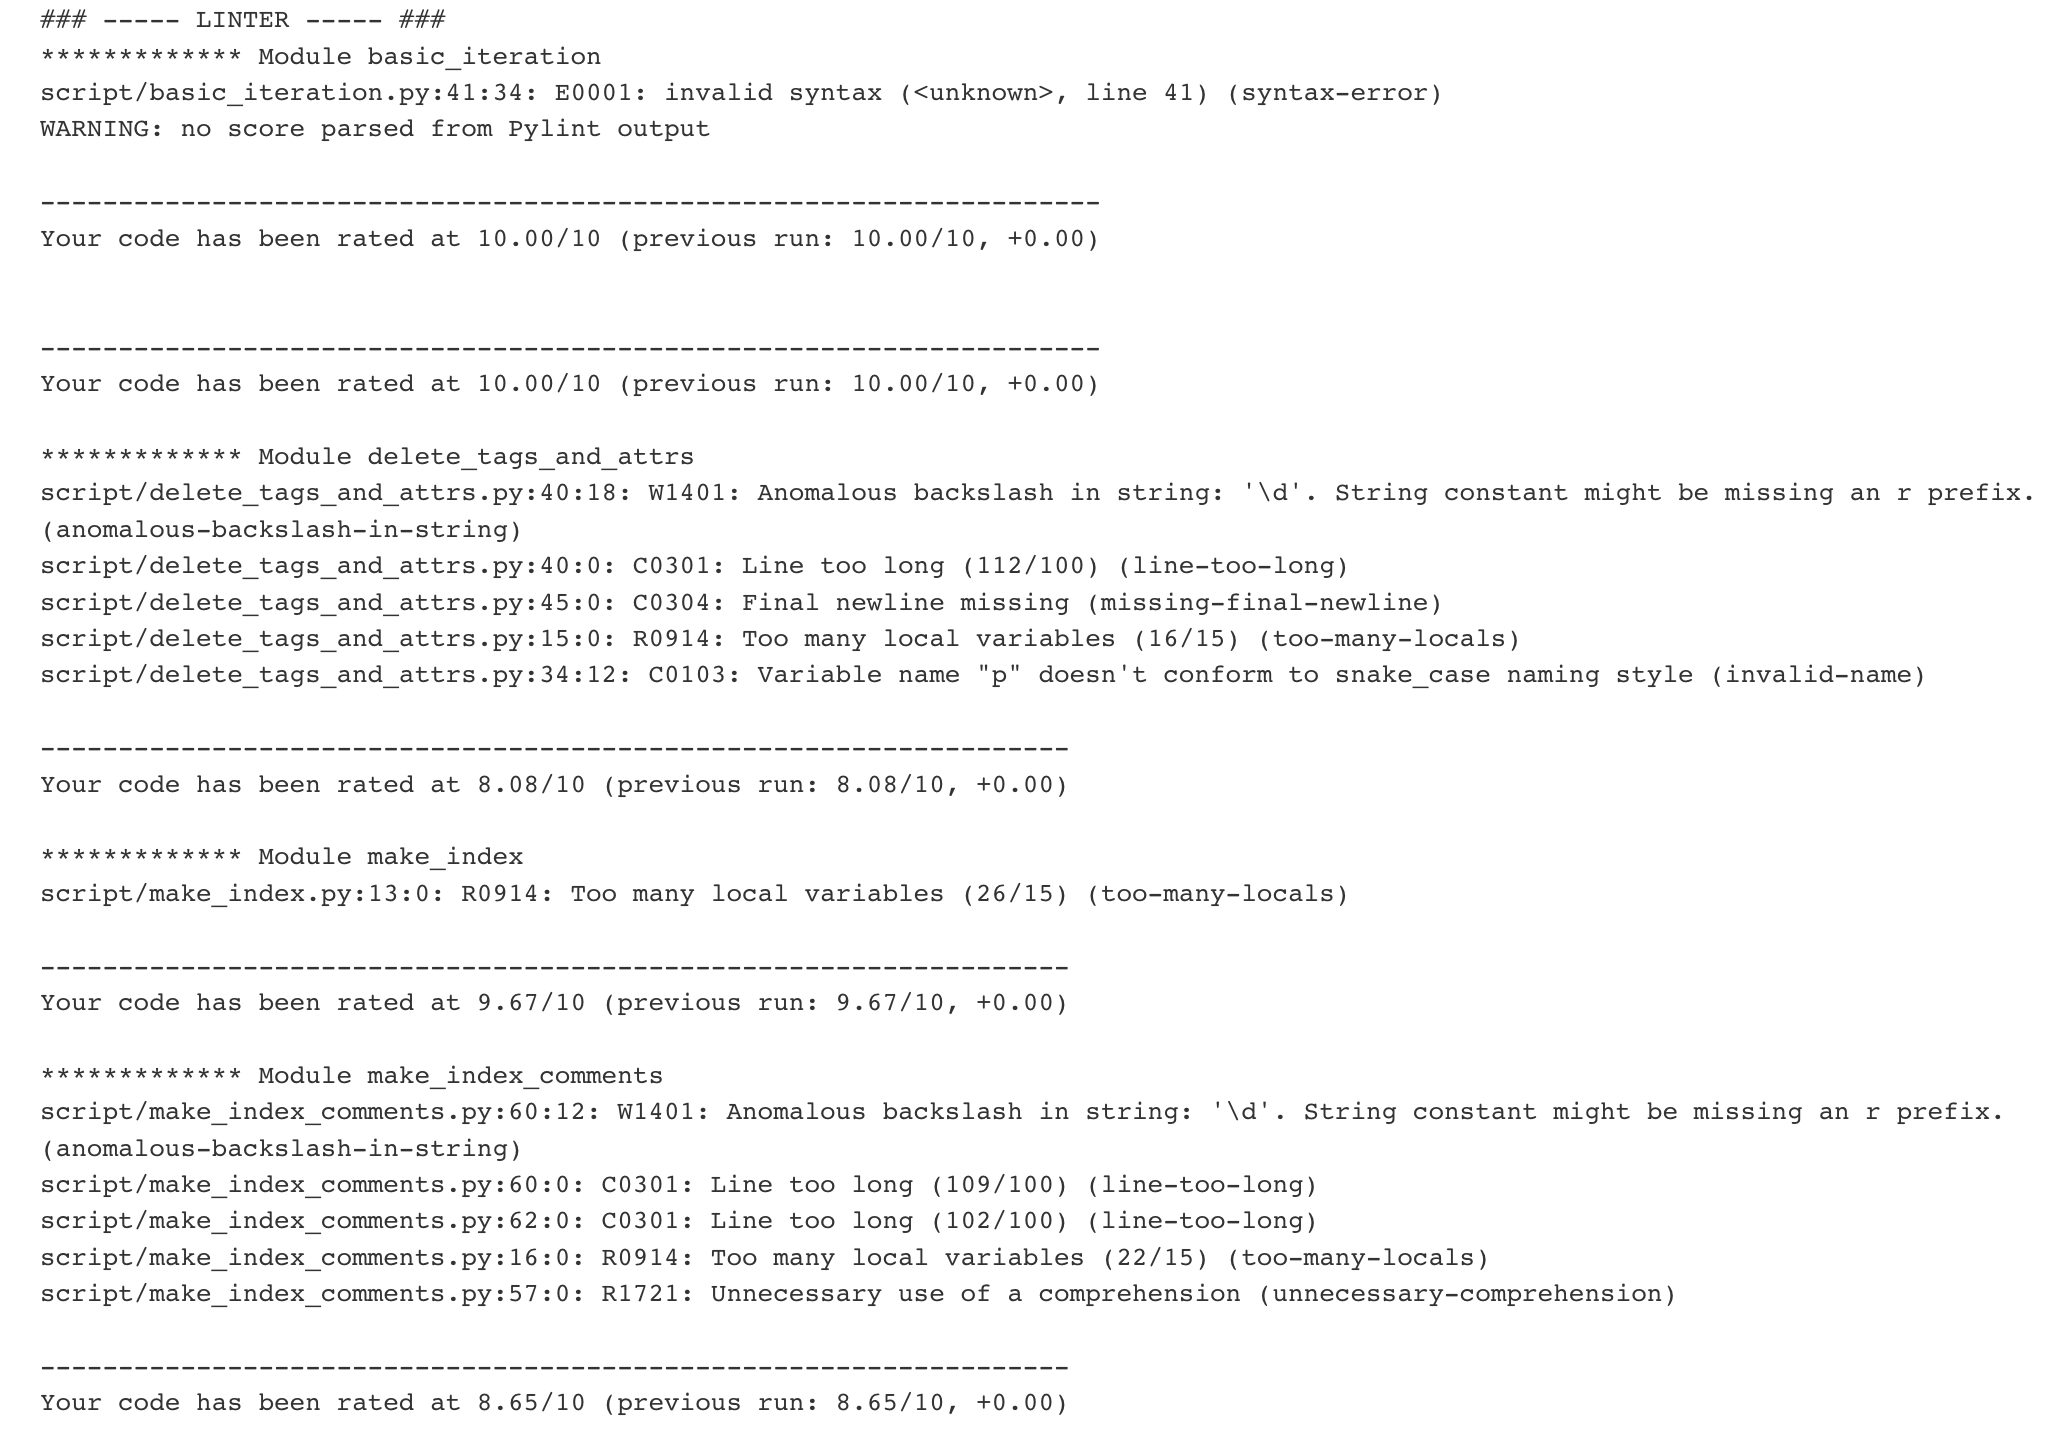
\includegraphics[width=15cm]{img/pylint_output.png}
    \caption[Exemple d'un contrôle de code par \textit{Pylint}]{Exemple d'un contrôle de code par \textit{Pylint}, qui donne une note à chaque script (\textit{module}) et détaille ensuite les erreurs détectées.}
    \label{fig:pylint}
\end{figure}

Le \textit{linter} \textit{Pylint} était également implanté dans le dépôt ; il s'agit d'un système de vérification de code Python. Son rôle est de contrôler à chaque \textit{push} la qualité du code des scripts, notamment la longueur des lignes, les intitulés des variables ou encore la documentation des fonctions. Le résultat est affiché dans une console sous forme de messages désignant le fichier concerné, la ligne de l'erreur et une désignation standardisée de celle-ci (\textit{line too long}, \textit{final newline missing}, etc. : \fig{} \ref{fig:pylint}).

\subsection{\pycharm{} et \oxygen}

Pour manipuler les fichiers XML, développer et activer les scripts Python, nous usions des logiciels \oxygen{} (éditeur de code XML sous licence propriétaire) et \pycharm{} (environnement de développement intégré pour la programmation en Python, une version est sous licence libre et une seconde sous licence propriétaire). 

Plusieurs fonctionnalités d'\oxygen{} ont facilité le traitement du corpus, notamment la possibilité de rassembler l'ensemble des fichiers dans un \og projet \fg. Par ce biais, des opérations --- par exemple effectuer une recherche ou remplacer une expression par une autre --- peuvent être menées sur le corpus sans requérir l'ouverture successive de chaque fichier. En outre, le logiciel dispose d'un système de validation du schéma du code, qui là encore peut être appliqué à tout le corpus à travers l'outil \og projet \fg.

\pycharm{} est équipé d'un outil de type \textit{linter} comparable à \textit{Pylint}, qui permet de s'assurer de la validité et de la lisibilité du code et facilite la programmation. \textit{Pylint} est cependant plus exigeant que le \textit{linter} natif de \pycharm, un double contrôle était donc nécessaire.

\section{Espaces de discussion}

La situation de confinement d'avril à mai et le maintien de la fermeture aux stagiaires des locaux d'Inria de juin à juillet a conduit à la mise en place d'outils de discussion.

\subsection{\Mattermost}

\Mattermost{} est un logiciel de discussion instantanée dont le code, écrit à l'origine sous un format propriétaire, a été publié en \opensource{}\footnote{Consultable sur \github{} (\url{https://github.com/mattermost/mattermost-server}, consulté le \today).} en 2015\footnote{Lindsay Brock, \textit{Open source Slack-alternative reaches 1.0: Self-host ready, Slack-compatible, MIT licensed}, 2 octobre 2015, \url{https://mattermost.com/blog/mattermost-3-4-16/} (consulté le \today).}. Auto-hébergé --- Inria stocke le code dans ses propres installations et n'a pas recours à un serveur distant ---, il s'agit de l'espace de discussion principal des agents d'Inria.

Composé de plusieurs \og chaînes \fg{} (\textit{public channels}) organisées de façon thématique, il leur permet d'échanger sur les différents projets et de suivre leur avancement, mais aussi d'exposer les difficultés techniques qu'ils rencontrent dans leur travail quotidien afin d'obtenir de l'aide. La chaîne \og \ocr \fg{} est ainsi fréquemment utilisée par les utilisateurs de \kraken{} (\fig{} \ref{fig:mattermost}).

\begin{figure}
    \centering
    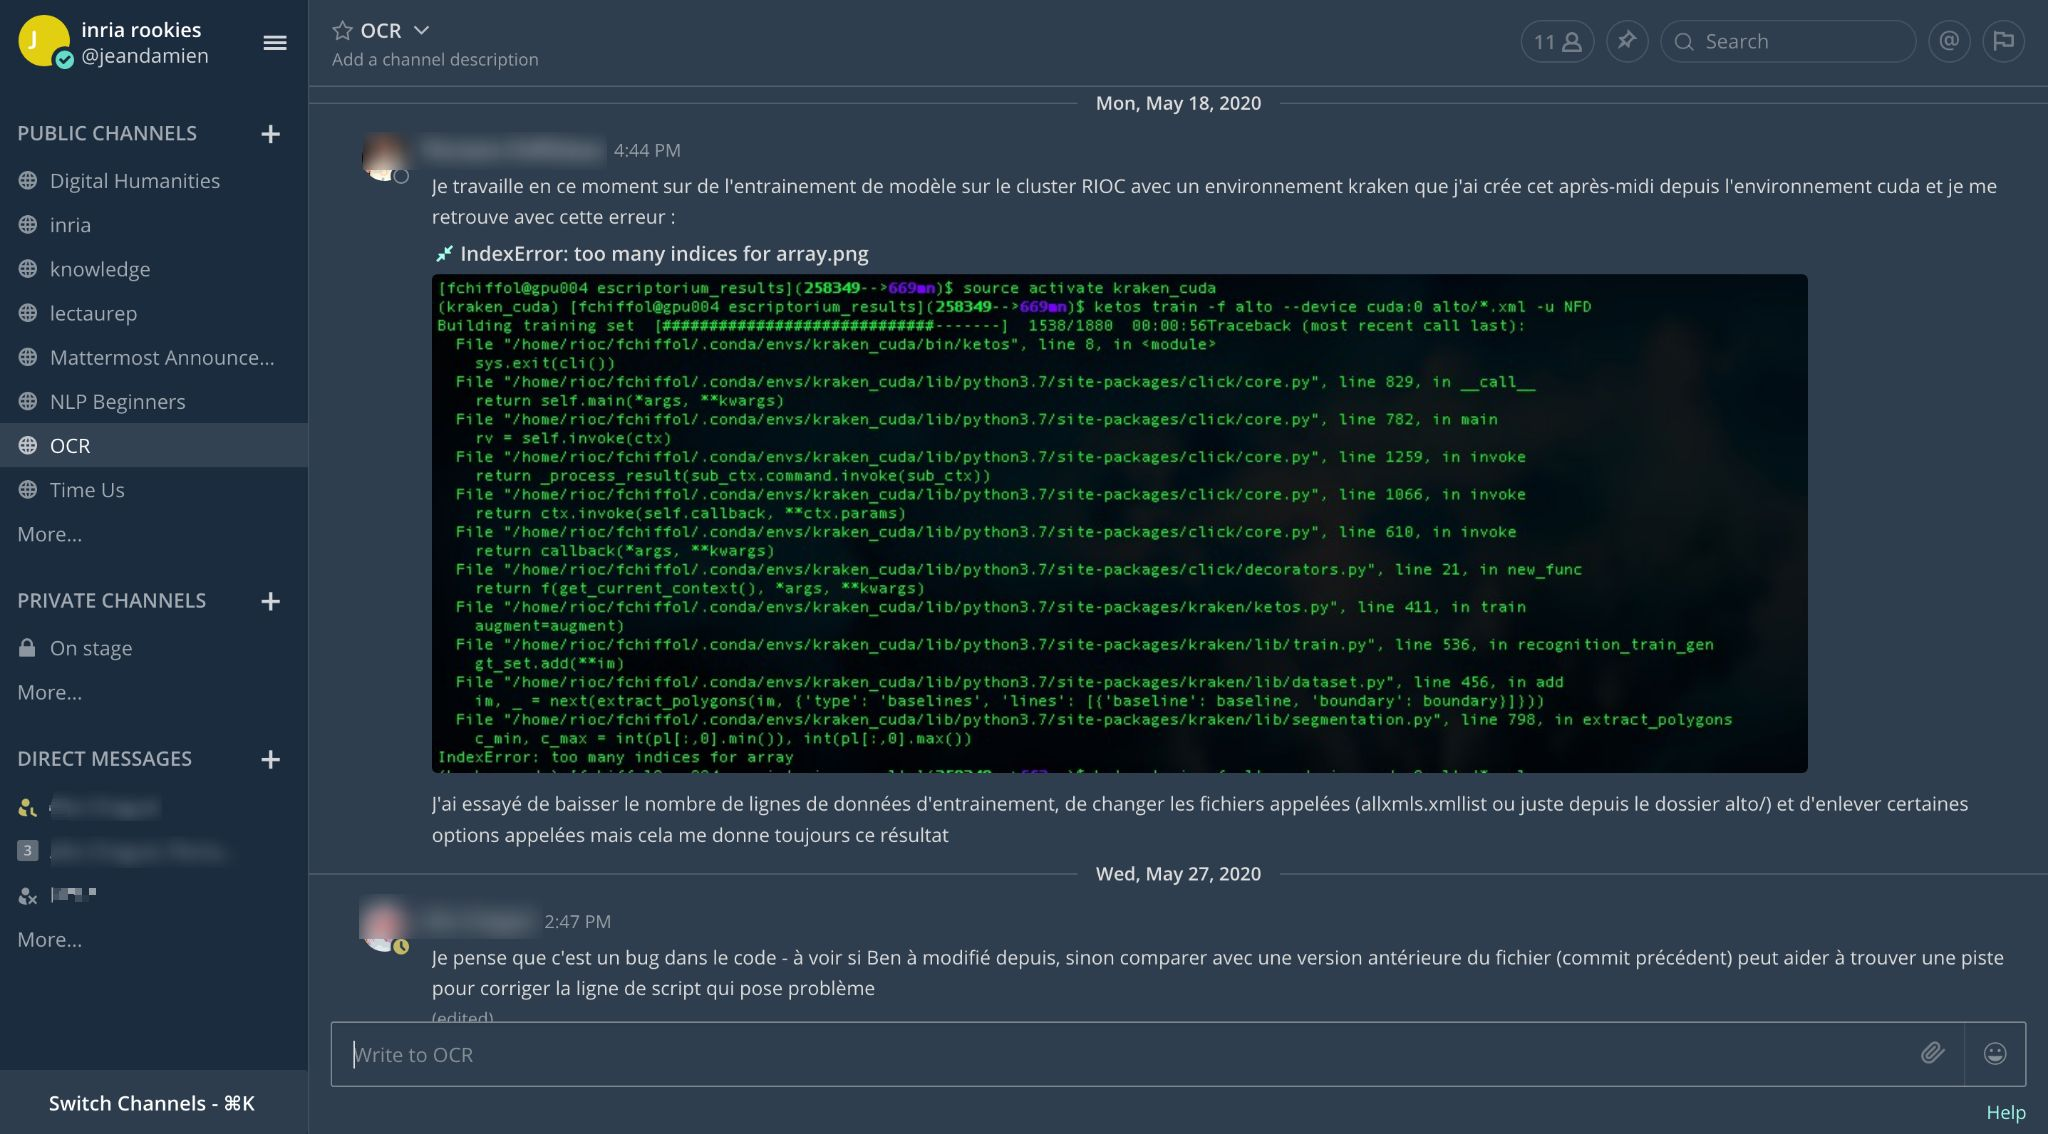
\includegraphics[width=16cm]{img/mattermost.jpg}
    \caption[\Mattermost{}]{Exemple de messages sur la chaîne \og \ocr \fg{} du \Mattermost{} d'Inria : une utilisatrice demande de l'aide au sujet d'une erreur dans l'exécution de \kraken{}. Sur le volet gauche se trouve la liste des chaînes disponibles.}
    \label{fig:mattermost}
\end{figure}

\subsection{\textit{Issues} et \mergerequests{} sur \gitlab}

Le programme \timeus{} possède également une chaîne ; cependant, pour les échanges afférents à nos missions, nous usions des espaces de discussion de \gitlab.

Les \issues{} et les \mergerequests{} n'ont en effet pas pour seule utilité de permettre aux utilisateurs d'exposer des problèmes ou de demander des fusions de branches. Il s'agit d'espaces dynamiques qui participent pleinement à la gestion de projet en offrant à ses participants la possibilité de donner leur avis ou d'apporter des solutions, par exemple pour résoudre un \textit{merge conflict}.

Cet aspect est facilité par l'usage du langage à balises \markdown\footnote{\gitlab{} use de sa propre version du \markdown, le \textit{GitLab Flavored Markdown} : \url{https://docs.gitlab.com/ee/user/markdown.html} (consulté le \today).}. Il permet une mise en forme légère (listes, liens hypertexte, diagrammes), ainsi qu'une intégration d'échantillons de code. Si ceux-ci ne sont pas fonctionnels, le \markdown{} permet de leur appliquer une coloration syntaxique, les rendant ainsi plus facile à lire (\fig{} \ref{fig:ex_gitlab}).

Les échanges sur ces espaces restent accessibles après la clôture des \issues{} ou des \mergerequests{}, constituant ainsi un historique de l'avancement du projet.

\begin{figure}
    \centering
    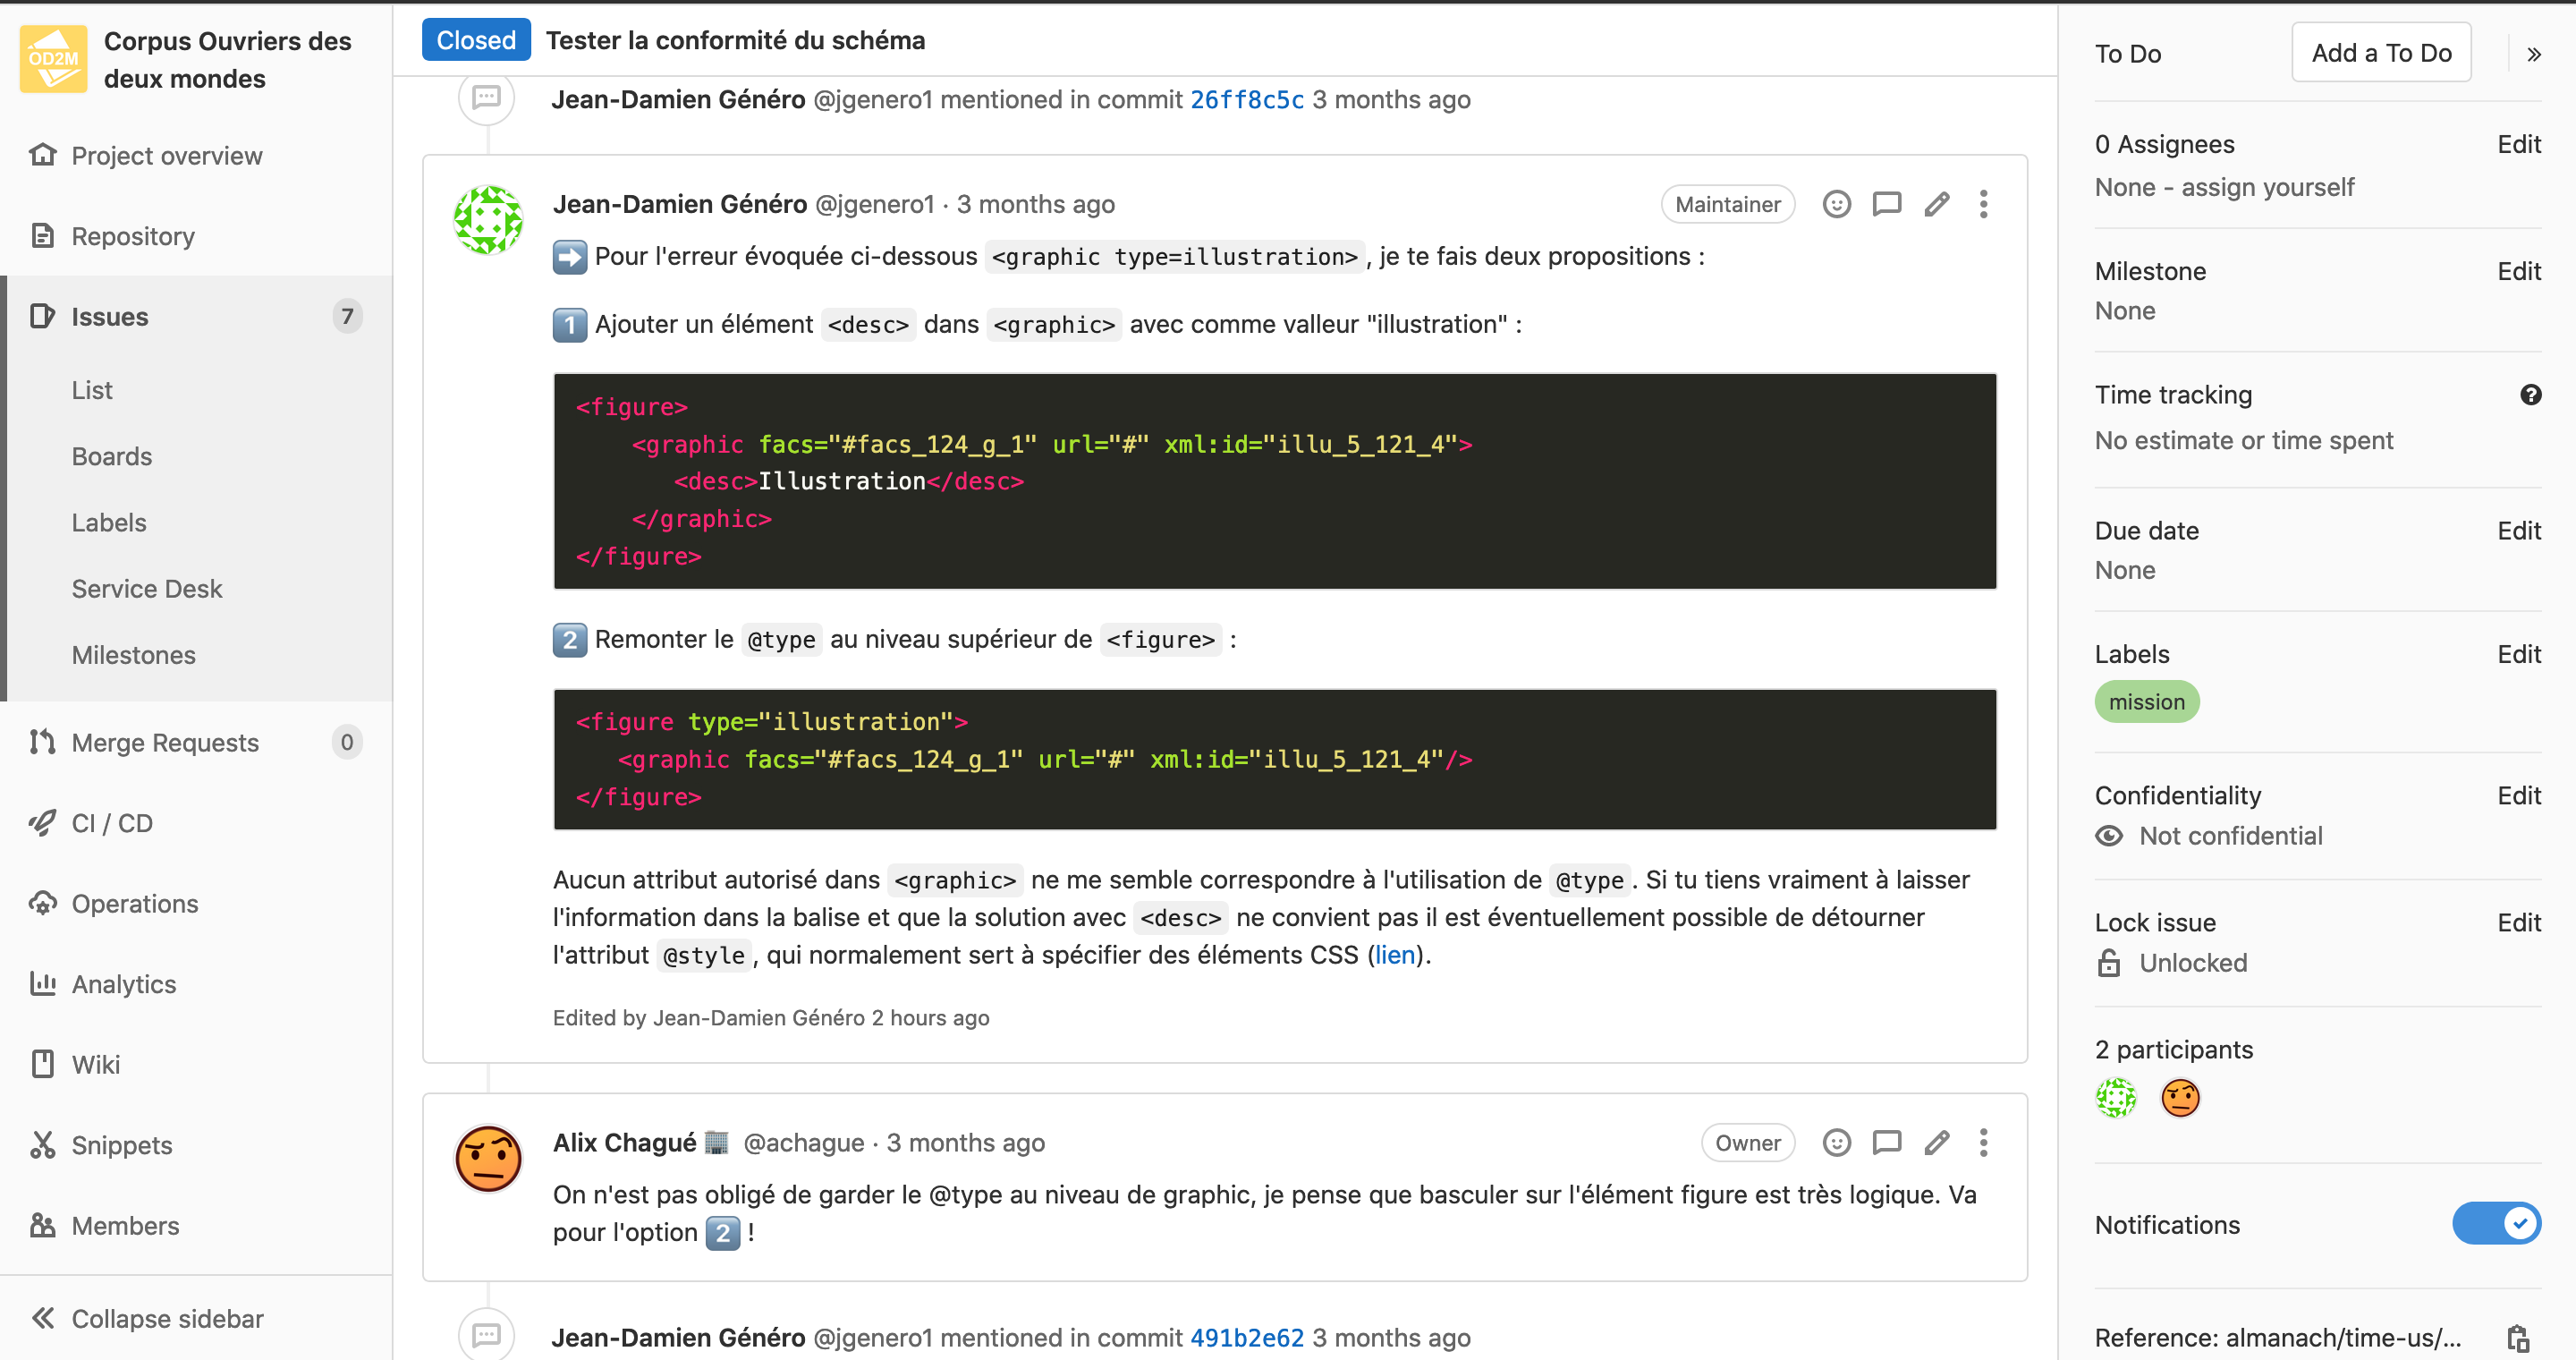
\includegraphics[width=16cm]{img/gitlab.png}
    \caption[Messages dans une \issue{} \gitlab]{Exemple de messages échangés avec une coloration syntaxique d'un code Python dans une \issue{} sur \gitlab.}
    \label{fig:ex_gitlab}
\end{figure}

\section{Feuille de route}

\subsection{Les missions du stage}

Au commencement de notre stage, huit \issues{} étaient ouvertes sur le \gitlab{} des \odm{}. Chacune correspondait à un problème ou à un point qui n'avait pas encore pu être développé. Elles constituaient donc notre \og feuille de route \fg, \cad{} l'exposé des missions que nous avions à réaliser (\ann{} \ref{ann:feuille_route}). Il nous a été demandé de les utiliser pour poser nos questions ou proposer nos solutions.

Les missions qui nous ont été confiées étaient de deux ordres.

Une première moitié consistait à contrôler les résultats du script \lse, tant au niveau du corpus qu'à celui de chaque fichier, et à effectuer des reprises si nécessaire. Tout d'abord, il s'agissait de détecter les erreurs de découpage des fichiers de volume et d'opérer les fusions ou les séparations nécessaires. Ceci avait pour but de donner à chaque fichier un identifiant unique après s'être assuré de l'unité de son contenu (\issue{}~1). Dans un second temps, nous devions nous intéresser à des éléments particuliers dans chaque fichier, à l'instar du contenu des balises \texttt{<facsimile>} (\issue{}~2), de la qualité des transcriptions (\issue{}~6) ou encore de la validité du schéma TEI (\issue{}~3); le contrôle de l'implémentation de la structure logique ayant constitué notre occupation principale.

L'autre moitié de nos missions avait pour but de valoriser les données des \odm{} en menant des actions ciblées. La principale consistait à identifier les individus enquêtés en liant les informations onomastiques du deuxième paragraphe (\textit{État civil de la famille}) à un tableau prosopographique établi par Stéphane Baciocchi, ingénieur de recherche du Centre de recherches historiques de l'EHESS (\issue{}~4). De plus, nous devions implémenter dans les fichiers un système permettant la citation de passages précis afin de faciliter les études des chercheurs et des chercheuses du programme en leur offrant la possibilité d'établir un lien direct entre leur travail et les données contenues dans les fichiers XML (\issue{}~5).

Il nous a enfin été demandé de publier sur le carnet de recherche en ligne de \timeus{} des billets rendant compte de notre travail\footnote{Carnet consultable à cette adresse : \url{https://timeus.hypotheses.org/}.}.

\subsection{Une gestion de projet ?}

Nous n'avons pas utilisé d'outil véritablement dédié à la gestion de projet, détournant plutôt un outil courant de \gitlab, les \issues.

Des fonctionnalités de \gitlab{} sont pourtant dédiées à une gestion plus fine. La principale est l'outil \og tableau de bord \fg{} (\textit{boards}). Par défaut, les \issues{} sont affichées sous la forme d'une liste présentant toutes celles qui sont ouvertes, deux onglets permettant d'accéder à celles qui ont été résolues ou bien de les afficher toutes. Avec l'outil \og tableau de bord \fg{}, l'utilisateur a accès à un tableau de quatre colonnes, la première listant les issues ouvertes, la seconde affichant une liste de tâches (\textit{todo list}), la troisième présentant les tâches en cours (\textit{doing}) et la dernières les \issues{} terminées.

Au-delà de la présentation des tâches, le tableau de bord est également interactif. Ainsi, sélectionner une \issue{} affiche ses métadonnées (agent en charge de sa résolution, labels, temps estimé, échéance). Un système de labels --- des étiquettes thématiques --- permet de classer les \issues{} et les tâches de la \textit{todo list}. Le tableau de bord offre donc une vision globale du projet selon une organisation chronologique, tout en permettant des vues synthétiques ciblées.

Le fonctionnement des \textit{boards} de \gitlab{} est comparable à celui d'autres applications, comme par exemple \textit{Trello}. Il s'agit d'un organisateur de tâche participatif, également sous forme de tableaux, qui est utilisé par ALMAnaCH et les Archives nationales pour coordonner le projet de lecture automatique des répertoires du Minutier central des notaires de Paris, LECTAUREP.

Pour autant, ces outils ne sont utilisés ni dans le cadre général du programme \timeus, ni dans le cadre particulier des \odm. Plusieurs raisons peuvent l'expliquer. En premier lieu, \timeus{} s'appuie sur une documentation dont le caractère disparate --- tant géographique que chronologique et typologique --- se heurte à toute volonté de gestion centralisée, d'autant que chaque membre est chargé de la gestion de sa documentation locale.

Un tel outil doit également être constamment maintenu à jour afin de garantir un gain de productivité. À l'échelle des \odm{} et de notre stage, le nombre relativement faible de missions (8) et d'intervenants (2) ne justifiaient pas la mise en place du tableau de bord \gitlab{} ou la création d'un \textit{Trello}. L'affichage basique des \issues{} sous forme d'une liste se suffisait à lui-même.

\newpage
\thispagestyle{empty}
\mbox{}
\newpage

\chapter{Contrôle du découpage des fichiers source}

\section{Les différents niveaux d'encodage}

Un document édité par le Consortium TEI, \textit{Best Practices for TEI in Libraries}, propose cinq niveaux d'encodage pour les documents TEI établis à partir de volumes imprimés tels que les \lodm\footcite[\textit{4.2. Encoding Levels}]{bestpratice}.

Le premier niveau est celui du découpage documentaire, soit la constitution d'un fichier qui reproduit le texte brut d'une unité codicologique et lui associe des métadonnées. Dans le cas des \odm, il s'agit du découpage des treize fichiers des volumes, qui ne s'est pas fait sans erreur, et de la constitution du \texttt{<teiHeader>}.

Le second niveau est celui dit de l'encodage \og minimal \fg, dont l'objectif est d'améliorer la navigation dans le document. Il s'agit d'identifier une structure physique, les pages du texte, délimitées par des balises \texttt{<pb>} entre lesquelles les paragraphes sont placés dans des \texttt{<p>}, et de la lier aux ensembles \texttt{<facsimile>} des images d'origine par un identifiant.

Le troisième niveau s'intéresse à la structure éditoriale, \cad{} à l'identification et à la reproduction de la structure hiérarchique du texte, en l'occurrence la structure initiée par Frédéric Le Play.

Le quatrième niveau est celui de l'encodage sémantique, destiné à mettre en valeur les éléments internes au texte afin d'en faire une production électronique autonome. Dans les fichiers des \odm, cela s'est traduit par l'élimination des éléments de mise en page des volumes tels que les en-têtes ou les numéros de page.

Le cinquième et dernier niveau est celui de l'annotation scientifique. Il s'agit par exemple de repérer et de mettre en valeur les éléments d'onomastique ou d'effectuer un traitement particulier pour les objets graphiques

Nous allons maintenant utiliser cette grille d'analyse afin de rendre compte des opérations de contrôle que nous avons menées. Notre travail ne s'est pas fait d'une manière aussi linéaire, et, dans les prochaines pages, nous allons totalement nous détacher de la chronologie du stage. 

Lorsqu'une correction était nécessaire, nous devions favoriser son automatisation par le biais d'un script Python. Cependant, ceci n’a pas toujours été possible, nous conduisant à engager des actions manuelles plus d'une fois.

\section{Vérification de la cohérence documentaire}

Le découpage des fichiers source a donné des résultats étonnants pour certains volumes. Ainsi, plus de trente fichiers avaient résulté du troisième volume de la deuxième série (\ann{} \ref{mappings2t3}).

Le contrôle a été opéré manuellement, par l'ouverture successive des fichiers. Les monographies devaient commencer par la reproduction de l'en-tête, point de repère du script \lse{} pour le découpage. Deux erreurs majeures ont été constatées.

\subsection{Erreur lors de la segmentation}

La première consistait en une erreur de découpage dans les précis \nos{}48~\textit{bis}\footcite{mono048b}, 66~\textit{bis}\footcite{mono066b} et 66~\textit{ter}\footcite{mono066c}. Le premier était scindé en dix fichiers contenant deux pages chacun (\texttt{s2t1\_cha\-pt\_6.xml} à \texttt{s2t1\_chapt\_15.xml}), le second et le troisième en respectivement sept et quatorze fichiers contenant quatre (\texttt{s2t3\_chapt\_7.xml} et \texttt{s2t3\_chapt\_8.xml} ; \texttt{s2t3\_chapt\_\-14.xml}) et deux pages (\texttt{s2t3\_chapt\_9.xml} à \texttt{s2t3\_chapt\_13.xml} ; \texttt{s2t3\_\-cha\-pt\_15.xml} à \texttt{s2t3\_chapt\_27.xml}). Lorsqu'il y avait deux pages, il s'agissait toujours d'un recto et d'un verso, et de deux rectos et deux versos lorsqu'il y en avait quatre.

Mis à part les premiers fichiers, qui commençaient par le titre du précis, les \texttt{<body>} de ces fichiers avaient un point commun : ils débutaient tous par les deux mêmes lignes, \texttt{<p>\textsc{précis de monographie}</p> \textbackslash n <p>[numéro de la page]</p>}. Or ces deux informations --- le rappel du titre du chapitre et le numéro de la page courante --- se trouvent sur une seule et même ligne dans les images. Une erreur de fission horizontale résultant d'une mauvaise segmentation s'était donc produite au moment de l'\ocr\footcite[p. 5-6]{karpinski}.

Dans son comportement normal, \lse{} est programmé pour détecter tout ce qui relève de l'en-tête ou du pied de page et le retirer afin de permettre une reconstitution optimale des paragraphes au moment de la transformation des fichiers XML pour une éventuelle édition. Ici, le script avait été dupé par l'erreur de segmentation : il n'avait pas vu des rappels de titre et des numéros de page, mais des titres et des numéros de chapitre. En conséquence, il avait opéré une coupure à cet endroit, \cad{} achevé le fichier en cours pour en amorcer un nouveau.

Une question demeure néanmoins : pourquoi trois des fichiers contenaient-ils quatre pages, à l'inverse des autres qui n'en contenaient que deux ? Les en-têtes des troisièmes pages avaient été détectés convenablement, et donc retirés du flux du texte. Aussi la séparation n'était-elle pas nécessaire.

L'erreur a été résolue par un transfert manuel du contenu de chaque fichier particulier dans un fichier global (\texttt{s2t1\_chapt\_6.xml}, \texttt{s2t3\_chapt\_7.xml} et \texttt{s2t3\_chapt\_14}). Le choix a été fait de ne pas modifier la numérotation des fichiers suivants, notamment afin de pouvoir effectuer un suivi sur la durée. C'est la raison pour laquelle, dans la deuxième série, le fichier \texttt{6} est suivi du \texttt{16} dans le premier volume et, dans le troisième, le  \texttt{7} par le \texttt{14}, lui-même précédant le \texttt{28} (\ann{} \ref{mappings2t1} et \ref{mappings2t3}, p. \pageref{mappings2t1}).

Cette opération a conduit à la suppression de vingt-huit fichiers. Ajoutons à cela le retrait de \texttt{s2t1\_chapt\_23.xml}, doublon de \texttt{s2t2\_chapt\_5.xml} : un total de vingt-neuf fichiers a été supprimé, ramenant le corpus de 223 à 194 unités.

\subsection{Défaut de transcription}

La seconde erreur majeure à laquelle nous avons été confrontés est le défaut d'une partie de la transcription dans six monographies (\ann{} \ref{ann:deficit-transcr}). Le titre et l'ensemble de la partie \textit{Observations préliminaires} manquent (\nos{}30\footcite{mono030a}, 33\footcite{mono033a}, 37\footcite{mono037a}, 44\footcite{mono044a}, 45\footcite{mono045a} et 46\footcite{mono046a}). Il ne s'agit pas d'une erreur de découpage, puisque déjà présente dans les treize fichiers source. C'est néanmoins l'opération de contrôle du découpage qui a permis de s'en rendre compte.

L'analyse de la mise en page et la segmentation se sont effectuées de manière convenable, comme en atteste la présence de \texttt{<facsimile>} entre le \texttt{<teiHeader>} et le \texttt{<text>}, repris des éléments \texttt{<TextBlock>} des fichiers ALTO d'origine. Néanmoins, les paragraphes 1 à 16, qui peuvent contenir des figures ou des tableaux mais sont principalement composés de textes, ont été considérés comme des éléments graphiques. En conséquence, chaque page est représentée par un élément \texttt{<figure>} contenant une balise \texttt{<graphic>} que l'attribut \texttt{@facs} relie à un \texttt{<facsimile>} ; \texttt{<pb>} venant signifier le changement de page (\fig{} \ref{fig:deficit}).

\begin{figure}[ht]
    \centering
    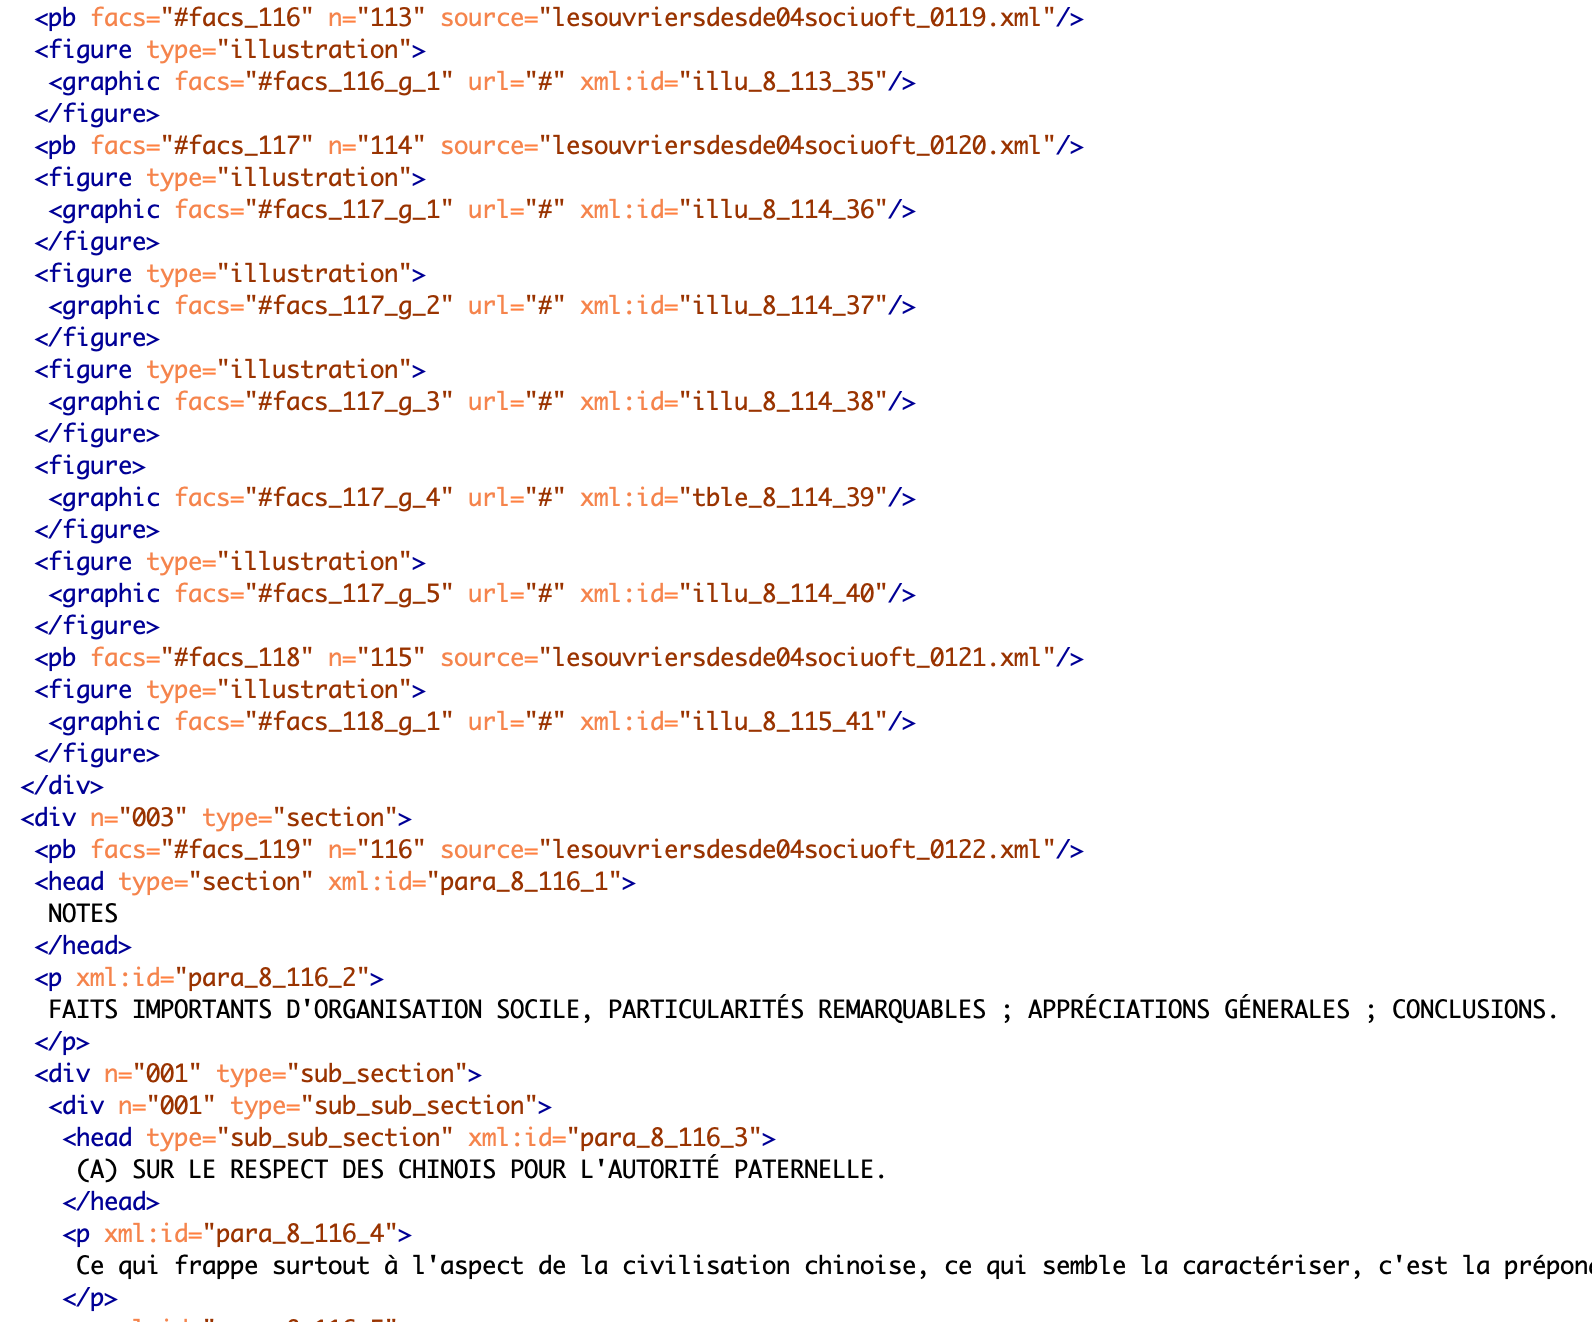
\includegraphics[width=16cm]{img/deficit_transcrip.png}
    \caption[Exemple d'un déficit de transcription]{Dans six fichiers, le contenu de la section \textit{Observations préliminaires} n'a pas été considéré comme du texte mais comme des figures. À l'inverse, la section \textit{Notes} a bien été prise en compte comme du texte. Exemple du fichier \texttt{s1t4\_chapt\_8.xml}.}
    \label{fig:deficit}
\end{figure}

Que s'est-il passé ? Le problème provient d'une fonction de \lse, \texttt{where\_do\_\-budgets\_start()}. Son  rôle est de déterminer l'index de la page où commencent les tableaux de budget et de placer cette donnée dans la variable \texttt{budget\_start}. Pour cela, il cherche la ligne \og \textsc{budget des recettes de l'année} \fg, qui se trouve entre l'en-tête de la page et la ligne supérieure délimitant le tableau de budget. Une fois cette information connue, le script sait que la page correspondante et les suivantes jusqu'au commencement de la section \textit{Notes} (index placé dans la variable \texttt{budget\_stop}) devront être considérées comme des objets graphiques.

Or les trois monographies concernées dans le quatrième volume (\nos{}30, 33 et 37) présentent un problème au niveau de la segmentation de la première page du budget. En effet, soit l'en-tête a été considéré comme du texte et le reste comme une illustration (\fig{}~\ref{fig:odm30tkb} et~\ref{fig:odm33tkb}), soit l'ensemble de la page a été considéré comme une illustration (\fig{}~\ref{fig:odm37tkb}). \kraken, à qui les zones de segmentation sont adressées, n'a donc rien à transcrire (à l'exception de la ligne d'en-tête dans deux cas), et \lse{} n'obtient pas de résultat quand il cherche la ligne \og \textsc{budget des recettes de l'année} \fg{}. La variable \texttt{budget\_start} est équivalente à \texttt{false} et \lse{} considère que les budgets débutent à la première page de la monographie. Il remplace alors toutes les transcriptions par des objets graphiques jusqu'aux \textit{Notes} qu'il traite normalement, et nous obtenons un fichier partiellement transcrit.

\begin{figure}[t]
    \centering
    \begin{subfigure}{0.3\textwidth}
     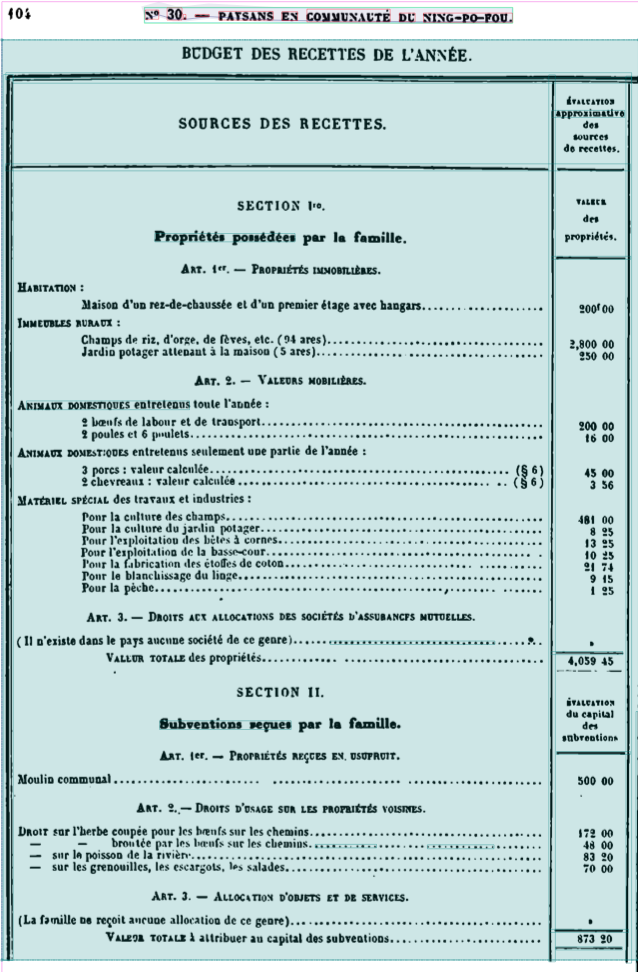
\includegraphics[width=1\linewidth]{img/transkribus_30.png}
     \caption{\no{}30, p. 104.}
     \label{fig:odm30tkb}
    \end{subfigure}
    \hspace{5pt}
    \begin{subfigure}{0.3\textwidth}
     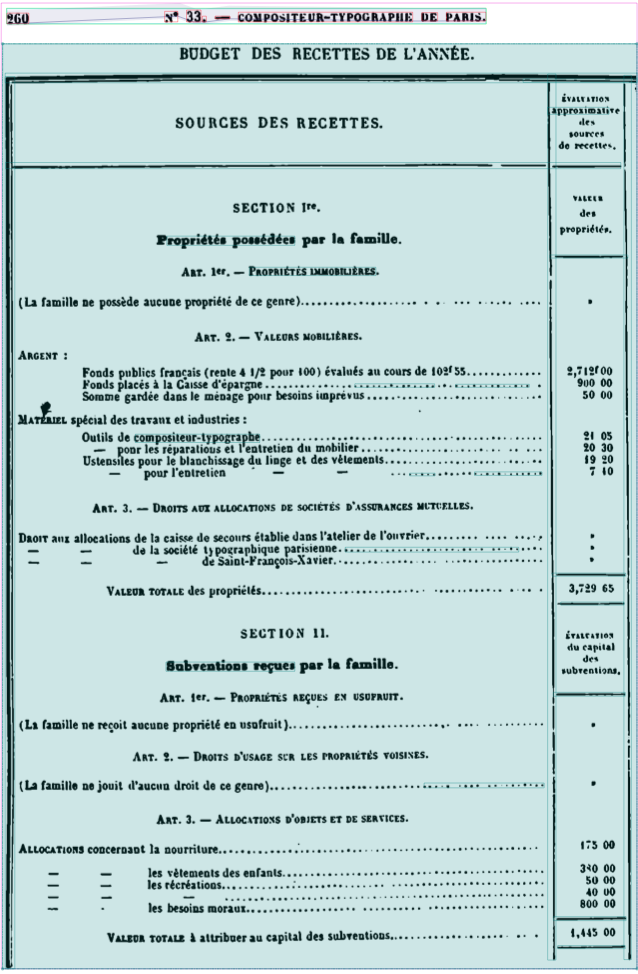
\includegraphics[width=1\linewidth]{img/transkribus_33.png}
     \caption{\no{}33, p. 260.}
     \label{fig:odm33tkb}
    \end{subfigure}
    \hspace{5pt}
    \begin{subfigure}{0.3\textwidth}
     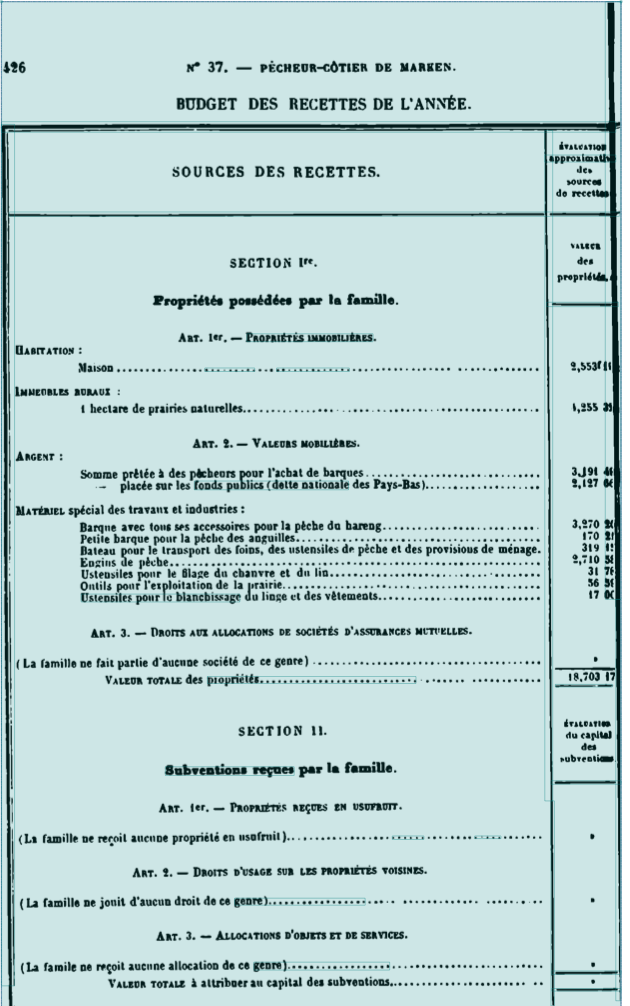
\includegraphics[width=1\linewidth]{img/transkribus_37.png}
     \caption{\no{}37, p. 426.}
     \label{fig:odm37tkb}
    \end{subfigure}
    \caption[Segmentation défectueuse dans \transkribus{}]{Segmentations dans \transkribus{} des pages liminaires des budgets des monographies \no{}30,  33 et 37. Dans les monographies 30 et 33, seul la ligne d'en-tête est considérée comme du texte.}
    \label{fig:odmtkbs1t4}
\end{figure}

Pour résoudre ce problème, une nouvelle \ocr{} et une nouvelle structuration sont nécessaires ; une correction par le biais d'une transcription manuelle ne fait en effet pas partie des possibilités acceptables pour l'équipe ALMAnaCH. Cette opération a été repoussée et nous n'avons pas eu à la mener. La reprise de ces six fichiers pourra cependant servir à valider les modifications apportées à \lse{} en tenant compte de l'ensemble des axes d'amélioration relevés au cours du stage et présentés dans ce mémoire. Notamment, l'éventualité de l'absence de valeur pour \texttt{budget\_start} pourrait 
être envisagée et traduite par un message d'erreur informant l'opérateur que le calibrage de la segmentation doit être changé.

\subsection{Cartographie, identification et inclusion}

\subsubsection{Cartographie}

Au-delà d'une vérification de la cohérence du découpage, cette étape de vérification avait pour but de reconnaître le contenu des fichiers, de leur associer un identifiant unique et de produire un fichier de cartographie ou \og \textit{mapping} \fg{} du corpus. Une partie des identifiants provenaient d'une bibliographie réalisée au format BibTeX\footnote{BibTeX est le logiciel de gestion de bibliographie du langage \LaTeX.} par Stéphane Baciocchi à partir de son exemplaire personnel du corpus.

Une partie seulement, car le fichier bibliographique ne s'intéressait qu'aux monographies, là où ALMAnaCH avait la volonté de travailler sur l'ensemble du corpus, monographies et fichiers de paratexte compris. Il a donc été nécessaire d'établir de nouveaux identifiants sur le modèle de ceux des monographies. Ces derniers se composent d'une série de trois chiffres suivie d'une lettre, \texttt{a} pour une monographie, \texttt{b} pour le précis \textit{bis} et \texttt{c} pour le \textit{ter} (\texttt{\textbackslash d\textbackslash d\textbackslash d[a-c]}). Pour poursuivre dans ce sens, nous avons choisi de donner au premier fichier de paratexte le numéro \texttt{401a} et de continuer jusqu'au dernier.

Trois versions de la cartographie ont été réalisées sous forme de tableaux CSV : la première contient uniquement les monographies, la seconde le paratexte et la troisième l'ensemble des fichiers\footnote{La troisième cartographie a été retravaillée afin de constituer l'annexe \ref{mapping} du présent mémoire.}. Chacune compte trois colonnes : identifiant du fichier, intitulé du fichier, titre du chapitre contenu dans le fichier.

\subsubsection{Identification}

Une fois les CSV constitués, il a fallu implanter les identifiants dans les fichiers TEI : il s'agissait de la première opération que nous avons pu automatiser. Après avoir relevé les identifiants et les libellés des fichiers dans le CSV général pour constituer un dictionnaire Python (\texttt{dict\_xml = \{'401a': 's1t1\_chapt\_1.xml', etc\}}), le script ouvrait chaque fichier un par un. À l'aide de la librairie \texttt{BeautifulSoup}, il analysait ensuite l'arbre XML (\fig{} \ref{fig:xmltree1}, p. \pageref{fig:xmltree1}) et implantait l'identifiant comme valeur de l'attribut \texttt{@xml:id} de \texttt{<TEI>} et de l'attribut \texttt{@ana} de la première \texttt{<div>}.

La première exécution de ce script a permis de faire remonter une erreur dans la constitution des identifiants : le XML ne permet pas qu'un \texttt{@xml:id} commence par un chiffre\footnote{\og \textit{Disallowed initial characters for Names include digits, diacritics, the full stop and the hyphen} \fg{}: \cite{xmlid}.}. Or il n'était pas possible de revenir sur ces identifiants, utilisés par d'autres chercheurs et chercheuses. La seule solution trouvée a été d'ajouter le préfixe \texttt{ID-} devant chaque identifiant afin de satisfaire aux règles de la TEI.

\begin{figure}
    \centering
    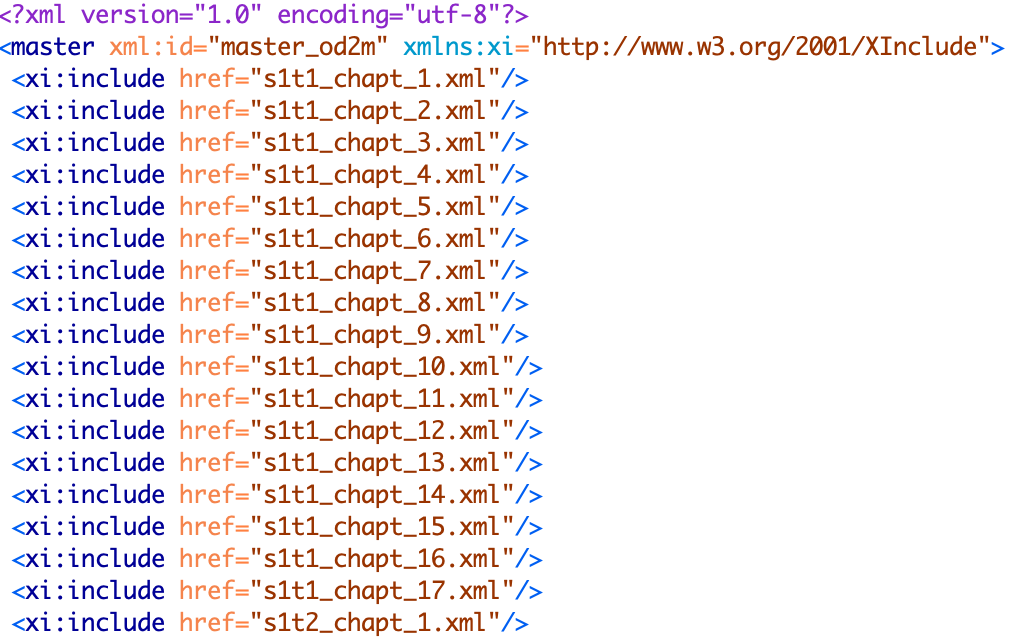
\includegraphics[width=15cm]{img/xinclude.png}
    \caption[Premières lignes du fichier \texttt{master.xml}]{Premières lignes du fichier \texttt{master.xml}. Dans la balise \texttt{<master>}, l'attribut \texttt{@xmlns:xi} contient l'adresse de l'espace de nom XInclude.}
    \label{fig:xinclude}
\end{figure}

\subsubsection{Inclusion}

ALMAnaCH souhaitait enfin pouvoir disposer d'un fichier XML regroupant l'ensemble des 194 fichiers. Pour cela, il nous a été demandé de recourir à un mécanisme d'inclusion grâce au langage XInclude, qui avait déjà été utilisé par le programme \timeus{} pour les fichiers de la documentation prud'homale.

Le principe est de constituer un fichier --- ici, \texttt{master.xml} --- dont le seul contenu est une balise \texttt{<master>} englobant une succession d'éléments \texttt{<xi:include>}. Ceux-ci possèdent un attribut \texttt{@href} contenant l'URI d'un fichier XML de paratexte ou de monographie. Il s'agit de l'identifiant uniforme d'une ressource (\textit{Uniform Resource Identifier}), \cad{} une séquence de caractères qui localise et nomme une ressource de manière pérenne\footnote{\og \textit{A URI is an identifier consisting of a sequence of characters matching the syntax rule named \texttt{<URI>}. It enables uniform identification of resources via a separately defined extensible set of naming schemes} \fg{} : RFC 3986, \textit{Uniform Resource Identifier (URI): Generic Syntax}, IETF, janvier 2005 (\url{https://tools.ietf.org/html/rfc3986}, consulté le \today).}.

Dans notre corpus, les URI des fichiers ne sont pas leurs identifiants mais le chemin qui conduit à eux : au moment d'analyser \texttt{master.xml}, le logiciel --- par exemple, \oxygen{} --- va lui adjoindre le contenu de la ressource localisée par la première URI, \cad{} le fichier \texttt{s1t1\_chapt\_1.xml}, qui contient la page de titre du premier volume, puis passer à l'URI suivante (le premier paratexte du premier volume), et ainsi de suite jusqu'au dernier fichier du troisième volume de la troisième série. Dans la mesure où \texttt{master.xml} et les fichiers TEI se trouvent dans le même dossier, le chemin est réduit aux seuls libellés de ceux-ci.

Ce fichier \texttt{master.xml} a été là encore constitué de manière automatique avec un script qui rassemble tous les libellés des fichiers dans une liste et, pour chacun d'eux, écrit la ligne \texttt{<xi:include href="[libellé]"/>} (\fig{} \ref{fig:xinclude}).

\section{Vérification de l'encodage minimal}

La mise en forme minimale des documents a été correctement exécutée par \lse, aucune partie de la transcription n'ayant été laissée sans encodage.

\begin{figure}[ht]
    \centering
    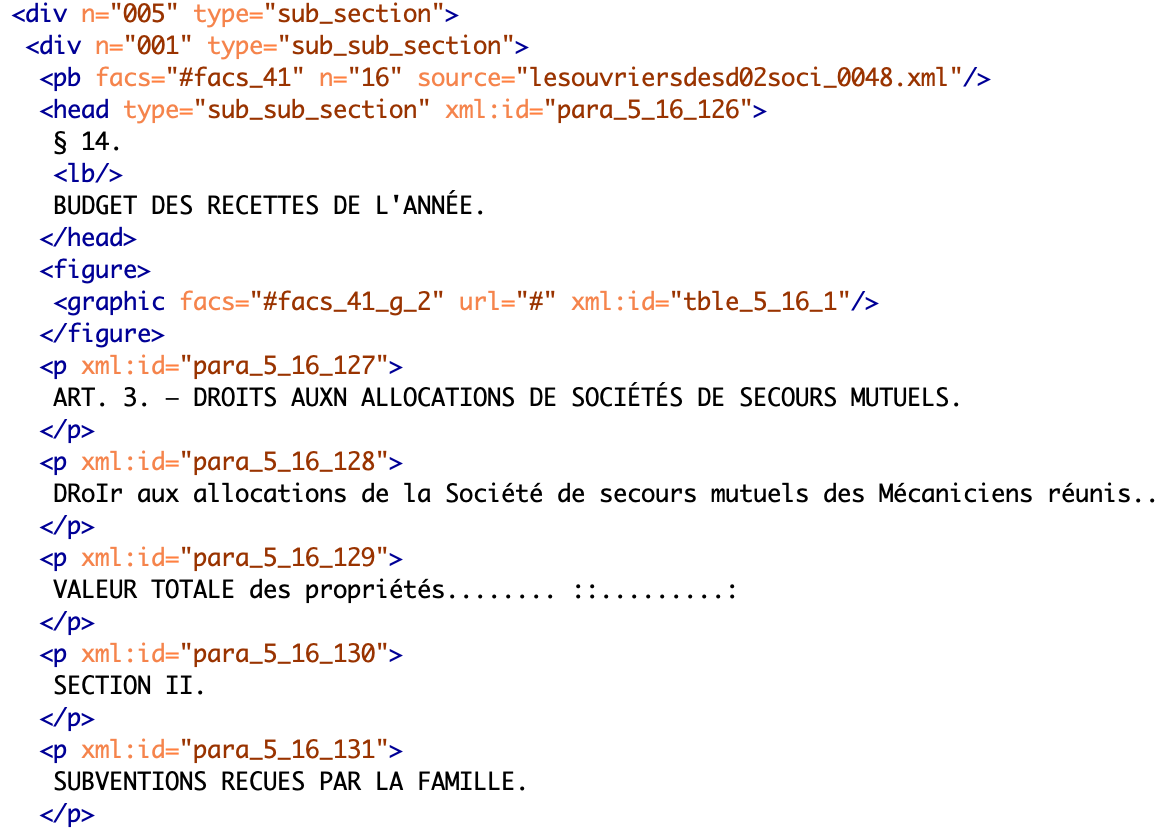
\includegraphics[width=15cm]{img/table_s2t2_chapt_5.png}
    \caption{Encodage du début du §14 de la monographie 56.}
    \label{fig:tableodm56xml}
\end{figure}

Les objets graphiques ont pu néanmoins poser problème au script. Nous avons vu dans la section précédente que dans six fichiers, toute une partie du texte avait été représentée par des éléments \texttt{<figure>}. L'inverse s'est également produit, \cad{} que des objets graphiques véritables --- à l'instar des tableaux de budget des paragraphes 14 à 16 --- ont souvent été considérés comme du texte. Ainsi, dans la monographie \no{}56\footcite{mono056a}, le tiers du premier tableau du paragraphe 14 est encodé dans un élément \texttt{<figure>} (articles 1 à 2), le reste, à partir de l'article 3, étant transcrit et placé dans des \texttt{<p>} (\fig{} \ref{fig:tableodm56xml}).

Pour autant, ces faits sont moins gênants que les cas inverses, dans la mesure où il s'agit de surplus de transcription. Les \texttt{<div>} encadrant ces sections de budgets étant en place, il est envisageable d'effacer automatiquement les balises \texttt{<head>} et \texttt{<p>} qu'elles contiennent et de n'ajouter que des \texttt{<graphic>} avec l'adresse de l'image de la page.

Cependant, toute mesure d'ajout ou de suppression d'élément \texttt{<p>} ou \texttt{<head>} a pour conséquence de rompre la logique interne du document. En effet, ces balises possèdent un attribut \texttt{@facs} dont la valeur renvoie à l'identifiant (\texttt{@xml:id}) d'un élément \texttt{<zone>} dans les \texttt{<facsimile>}.

Pousser la précision de ces derniers jusqu'au niveau des paragraphes devient inutile puisque la correspondance entre les \texttt{<zone>} et les \texttt{<p>} ou les \texttt{<head>} ne peut plus 
être garantie. De fait, le niveau de référence devient la page (\texttt{<surface>}) et non le paragraphe. Les nombreuses modifications que nous avons menées sur ces balises nous ont donc conduit à retirer l'ensemble des éléments \texttt{<zone>} et des attributs \texttt{@facs} des paragraphes et des titres par le biais d'un script. Ce dernier a effectué un ensemble de 138263 suppressions de ligne dans le corpus. Dans l'arbre XML de départ (\fig{} \ref{fig:xmltree1} p. \pageref{fig:xmltree1}), le seul descendant de l'élément \texttt{<surface>} est désormais \texttt{<graphic>}.

\newpage
\thispagestyle{empty}
\mbox{}
\newpage

\chapter[Découpages éditorial et sémantique]{Contrôle des découpages éditorial et sémantique}

Le contrôle du découpage éditorial, \cad{} de l'implémentation de la structure logique, a donné lieu à la reprise la plus importante. Il s'agit d'un point crucial pour les fichiers des \odm, du fait de l'importance accordée par l'école leplaysienne à une structure logique qui seule permet de transformer les \og faits observés \fg{} sur le terrain en des \og faits décrits \fg{} par la monographie\footcite[p. 87]{baciocchi2}.

Un exemple de l'encodage attendu se trouve dans l'annexe \ref{ann:encodage-structure}.

\section{Découpage éditorial}

\subsection{Niveau des titres (\texttt{<head>})}

Pour commencer, nous avons cherché à évaluer l'étendue des corrections à effectuer à l'aide d'un script. Nous n'avons pas eu recours à un schéma de validation pour détecter les erreurs car certaines étaient de type documentaire (titre mal orthographié notamment) et n'affectaient pas la validation du fichier. Un schéma n'aurait donc pas été capable de les détecter.

Le script comparait une structure idéale --- \cad{} l'idée que chaque fichier de monographie devait contenir dans des \texttt{<head>} deux titres de niveau section (B et C), quatre titres de sous-section (I à IV) et seize titres de paragraphes (§1 à §16, \cf{} \ann{} \ref{structure}) --- à la structure réelle contenue les fichiers. Les titres qui n'avaient pas été trouvés étaient listés en sortie.

Plus de quatre cent cinquante erreurs ont été identifiées. Ce chiffre comptait de nombreux faux positifs en raison de la non-prise en compte de la qualité des transcriptions. Certains titres étaient en effet présents mais leurs transcriptions étaient fautives. Nous avons contrôlé chaque signalement avec Alix Chagué, et complété un \textit{Google Drive} afin de réaliser une typologie des erreurs :

\begin{itemize}
    \item Des distances d'édition trop faible entre deux titres avaient causé le remplacement de l'un par l'autre :
    \begin{itemize}
        \item (II.) \og Mode d'existence de la famille \fg{} par (III.) \og Moyens d'existence de la famille \fg.
        \item \og § 11. -- Récréations \fg{} par \og § 7. -- Subventions \fg.
    \end{itemize}
    \item La monographie \no{}44\footcite{mono044a} est la dernière à posséder des titres de paragraphe sur une seule ligne, un retour à la ligne étant ensuite systématiquement effectué entre le numéro et le libellé du paragraphe (\fig{} \ref{fig:titre8}. Cet élément n'avait pas été compris par \lse, qui a pu répéter ou non le numéro du paragraphe sur la ligne du libellé.
    \begin{itemize}
        \item En cas de répétition, le numéro original était placé dans un \texttt{<p>} et le titre avec le numéro ajouté dans un \texttt{<head>} (\fig{} \ref{fig:ex_structure} p. \pageref{fig:ex_structure}).
        \item En cas de non répétition, le titre n'était pas toujours détecté et les deux lignes étaient encodées dans des \texttt{<p>}.
    \end{itemize}
    \item Des titres transcrits avec une distance trop importante par rapport au modèle n'avaient pas été détectés.
    \item Les titres des tableaux de budgets étaient souvent transcrits plus d'une fois.
    \item Les cas particuliers n'avaient pas été pris en compte :
    \begin{itemize}
        \item La monographie porte sur un ouvrier ou une ouvrière et non pas une famille, ce qui conduit à un changement dans la terminologie (par exemple, \og État civil de la famille \fg{} devient \og État civil de l'ouvrier \fg) : concerne notamment \texttt{s1t2\_chapt\_4.xml}, \texttt{s1t3\_chapt\_7.xml} et \texttt{10} ;
        \item Certains titres de paragraphe n'étaient pas séparés du texte mais imprimés en italique au début de celui-ci (\fig{} \ref{fig:titre8_66b} et \ann{} \ref{ann:structure-allegee}) ;
        \item Le titre n'est pas imprimé (\ann{} \ref{ann:titre-non-imprimes}, \ref{ann:structure-allegee} et \ref{ann:no-notes-no-16}) ;
        \item La monographie possède une structure qui lui est propre (\ann{} \ref{ann:remarques-et-cas-particuliers}).
        \item La sous-section des budgets est titrée dans huit monographies, mais ce titre n'a jamais été détecté comme tel par \lse.
    \end{itemize}
\end{itemize}

\begin{figure}[t]
    \centering
    \begin{subfigure}{0.4\textwidth}
     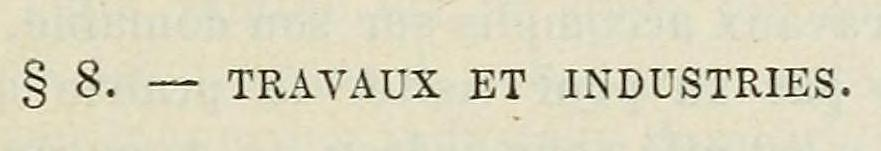
\includegraphics[width=1\linewidth]{img/titre_8_mono_44_p_327.jpg}
     \caption{\no{}44, p. 327.}
     \label{fig:titre8_44}
    \end{subfigure}
    \hspace{5pt}
    \begin{subfigure}{0.3\textwidth}
     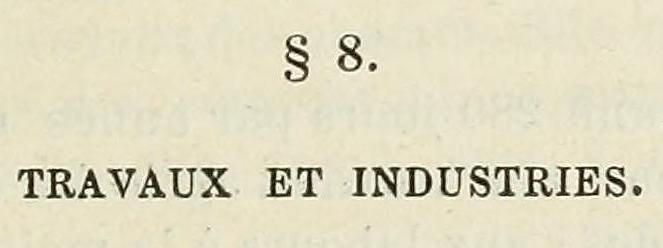
\includegraphics[width=1\linewidth]{img/titre_8_mono_45_p_399.jpg}
     \caption{\no{}45, p. 399.}
     \label{fig:titre8_45}
    \end{subfigure}
    \begin{subfigure}{0.8\textwidth}
     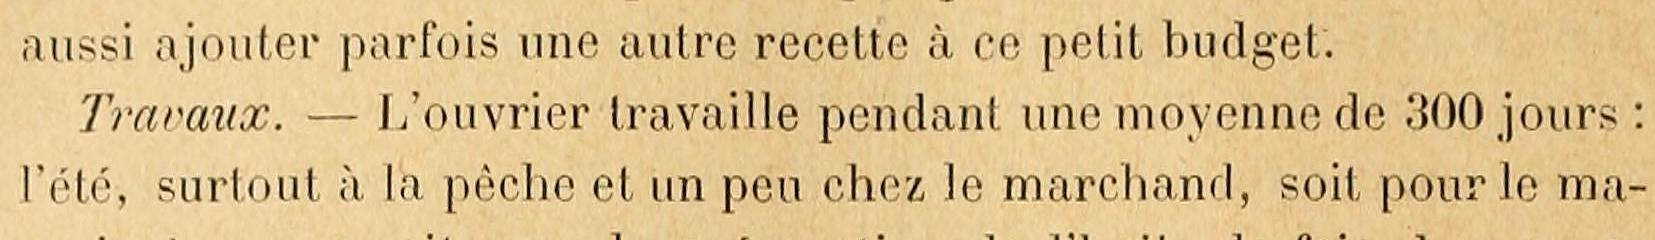
\includegraphics[width=1\linewidth]{img/titre_8_mono_66_p_130.jpg}
     \caption{\no{}66, p. 130.}
     \label{fig:titre8_66b}
    \end{subfigure}
    \caption[Comparaison entre les titres 8 des monographies \nos{}44, 45 et 66 \textit{bis}.]{Comparaison entre le titre 8 de la monographie \no{}44, sur une seule ligne (a), et celui de la monographie suivante, sur deux lignes (b). Dans la monographie \no{}66 \textit{bis} (c), le titre est placé en italique au début du paragraphe.}
    \label{fig:titre8}
\end{figure}

\subsection{Niveau des divisions (\texttt{<div>})}

L'implémentation de la structure logique ne s'est pas uniquement traduite par une mise en forme des titres : chaque \texttt{<head>} est en effet attaché à une \texttt{<div>} (\fig{} \ref{fig:deficit} p. \pageref{fig:deficit}). Tous deux possèdent un identifiant \texttt{@type} qui définit leur niveau (\texttt{section}, \texttt{sub\_section} ou \texttt{sub\_sub\_section}), la \texttt{<div>} étant en plus nantie d'un numéro (\texttt{@n}).

Trois erreurs ont été constatées à ce niveau :

\begin{itemize}
    \item Lorsqu'un titre n'était pas détecté, la \texttt{<div>} correspondante n'était pas créée et le paragraphe était intégré dans la division précédente, invalidant de fait l'ensemble de la numérotation ;
    \item Des \texttt{<div>} surnuméraires ont été implantées (\fig{} \ref{fig:ex_structure} p. \pageref{fig:ex_structure}) ;
    \item Au cour du stage, il a été décidé de placer le titre de la monographie dans une \texttt{<div>} de type \texttt{section}, ce qui impliquait une reprise dans l'ensemble des fichiers.
\end{itemize}

\subsection{\textit{Tabula rasa}}

Le nombre élevé de cas particuliers rendait impossible une automatisation complète de cette reprise. Nous allons d'abord exposer la méthode suivie pour le traitement des cas particuliers avant de rendre compte de celle utilisée pour le reste du corpus.

\subsubsection{Cas particuliers}

Les monographies d'ateliers (\texttt{s3t1\_chapt\_2.xml}\footcite{mono472a} et \texttt{s3t2\_chapt\_10.xml}\footcite{mono473a}) imposaient une reprise manuelle du fait de leur structure unique. De plus, dans ces fichiers, ainsi que dans certaines monographies de familles, plusieurs titres n'étaient pas détachés des paragraphes (\fig{} \ref{fig:titre8_66b}). Le recours à la balise \texttt{<head>} n'était pas possible pour les traiter, dans la mesure où elle constitue normalement un bloc séparé des \texttt{<p>}. Plusieurs solutions, toutes insatisfaisantes, ont été envisagées.

La plus légère consistait à signaler la mise en forme de ces titres (italique ou gras) par des balises de mise en valeur telles que \texttt{<emph style="italic">} ou \texttt{<hi rend="i">}. Nous n'avons pas opté pour ce choix en raison des règles de la TEI qui ne prévoient pas d'attributs pour caractériser ces balises (notamment, \texttt{@type}). Aussi n'aurait-il pas été possible de les différencier d'autres passages possédant une mise en forme similaire dans le corps du texte lors de la transformation des fichiers XML en d’autres formats.

Une deuxième solution, beaucoup plus lourde pour le fichier, aurait consisté en l'imbrication de  \texttt{<div>}. Le \texttt{@type} assigné à la division aurait permis de savoir que le \texttt{<head>} et le \texttt{<p>}, eux-même placés dans une sous-division, ne constituaient qu'un seul paragraphe dans le volume original (\fig{} \ref{fig:solution2}). La contre-partie est que chaque paragraphe aurait dû être placé dans une sous-division.

\begin{figure}[ht]
    \centering
    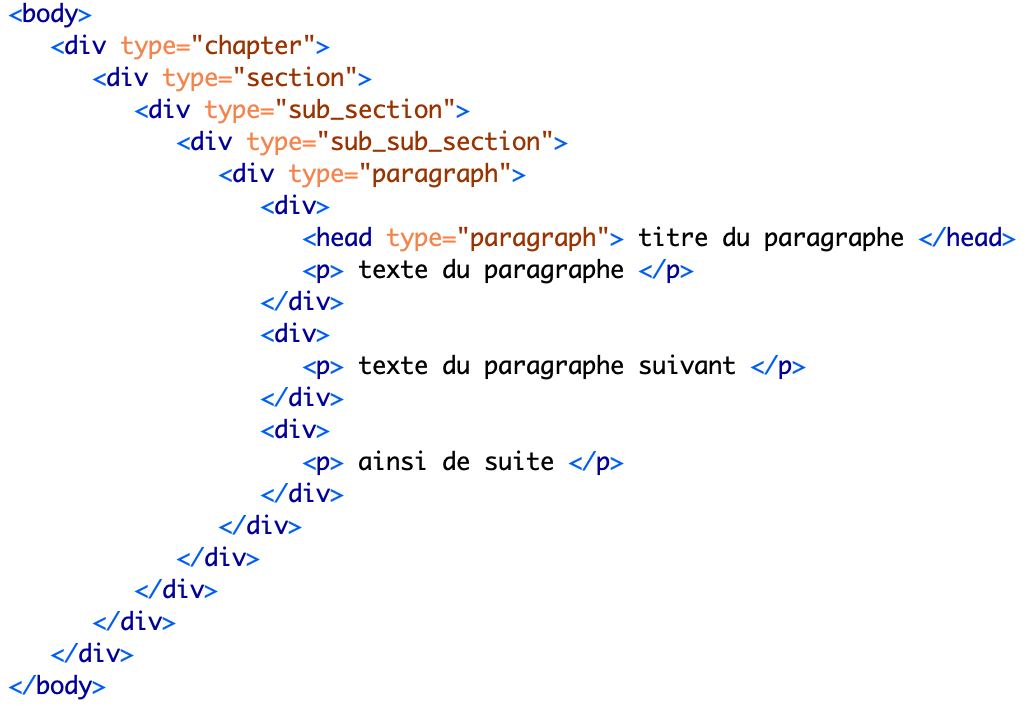
\includegraphics[width=15cm]{img/solution2.png}
    \caption[Proposition pour un encodage des paragraphes.]{Représentation de la deuxième solution, dont le résultat est de produire une imbrication malvenue de \texttt{<div>}.}
    \label{fig:solution2}
\end{figure}

Au final, \timeus{} n'a opté pour aucune solution, considérant que le nombre de cas était suffisamment bas pour ne pas avoir à mettre en place une solution particulière. Pour autant, cette décision n'a pas eu pour effet d'arrêter le niveau de granularité des titres à la sous-sous-section.

En effet, les fichiers \texttt{s1t5\_chapt\_9.xml}\footcite{mono041a} et \texttt{10}\footcite{mono042a} comprennent des précis de monographie dotés de leur propre structure logique et intégrés dans le corps de leurs sections \textit{Notes} (\fig{} \ref{fig:precis41}). Les titres étant détachés des paragraphes, il a été possible de mobiliser un niveau inférieur à la sous-sous-section, le \texttt{paragraph}, afin de rendre compte de cette structuration.

\begin{figure}
    \centering
    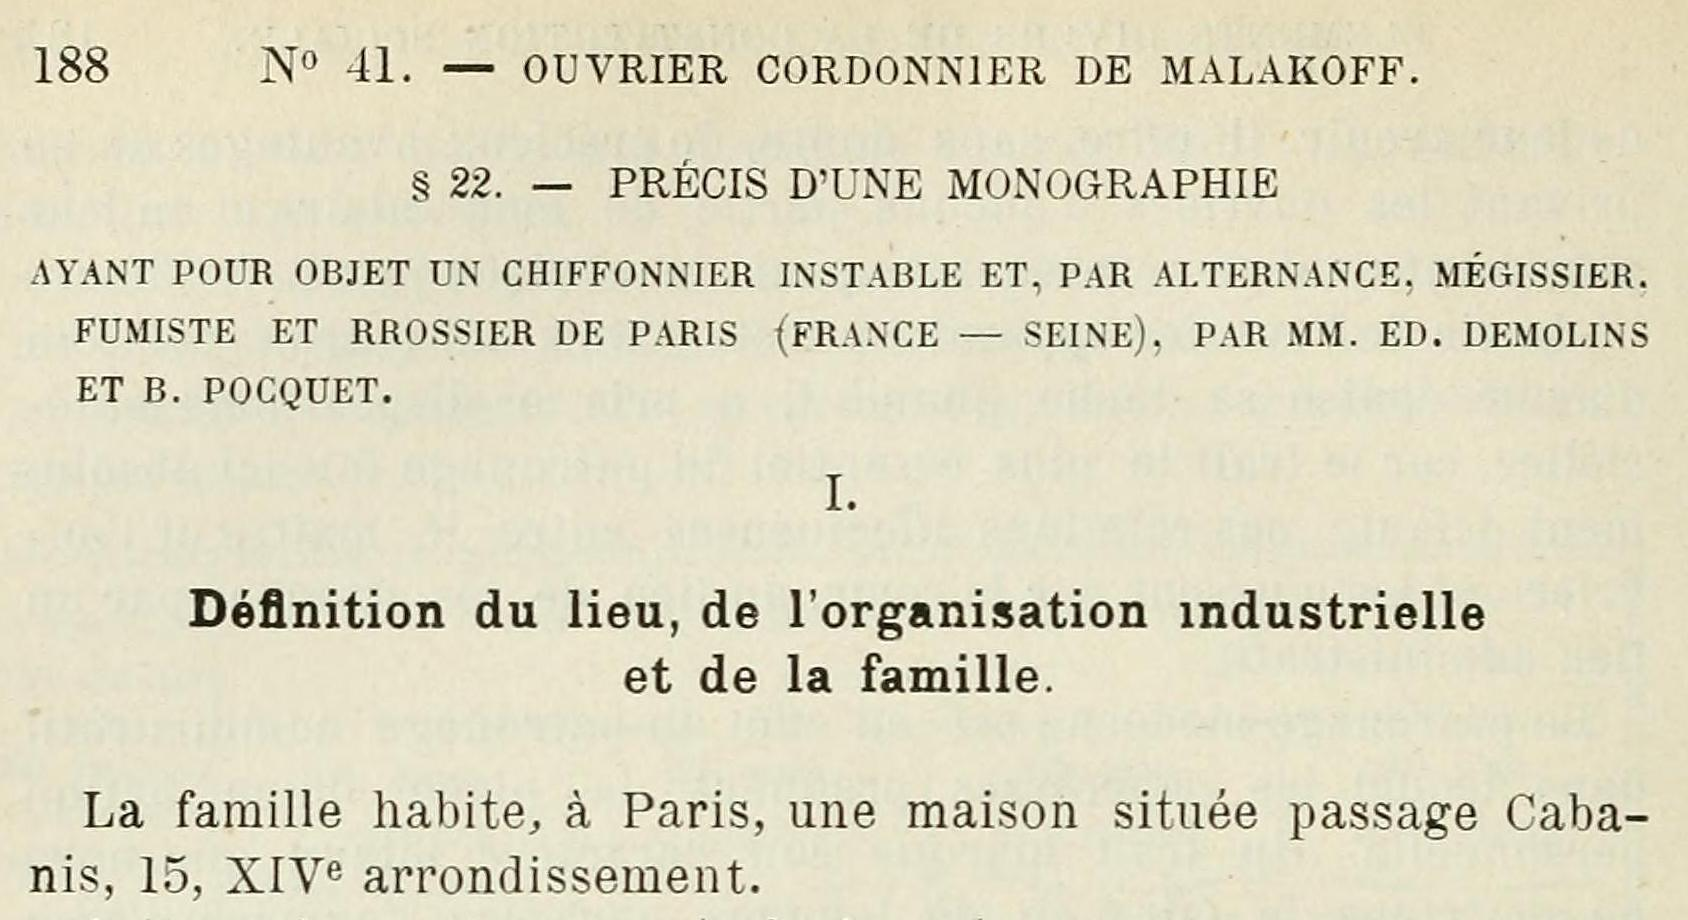
\includegraphics[width=14cm]{img/precis_mono_41_p_188.jpg}
    \caption[Précis de monographie dans la monographie \no{}41.]{La monographie \no{}41 compte un précis de monographie intégré en tant que paragraphe de sa section \textit{Notes}. À partir de la deuxième série, les précis sont toujours séparés de leurs monographies.}
    \label{fig:precis41}
\end{figure}

\subsubsection{Reconstruction de la structure}

Ces cas particuliers réglés, il restait à prendre en charge l'essentiel du corpus, \cad{} une soixantaine de monographies. Une reprise entièrement manuelle n'était pas envisageable en raison du temps trop important qu'elle aurait nécessité. À l'inverse, une automatisation totale aurait nécessité une longue étude et un relevé minutieux des aléas de la détection et de la transcription des titres.

Nous avons donc choisi d'implanter la structure logique par des cascades d'expressions régulières appliquées sur un lot de fichiers à l'aide d'un script. Les expressions régulières sont des motifs qui permettent de décrire des chaînes de caractères dans un texte. Le module \texttt{re} de Python permet de mobiliser ces expressions dans un script, et notamment d'effectuer des substitutions grâce à la fonction \texttt{re.sub()}.

Du fait de la désorganisation massive des \texttt{<div>}, la première expression régulière consistait à faire table rase de ces balises. Le script reconstruisait ensuite la structure en progressant selon ses niveaux. Il commençait par implanter la \texttt{<div>} de type \texttt{chapter} et celle de la première section (la page de titre). Venaient ensuite les \texttt{<div>} des deux sections restantes (\textit{Observations préliminaires} et \textit{Notes}), puis celles des sous-sections, etc.

Les expressions régulières recherchaient les libellés des titres lorsqu'il s'agissait de sections ou de sous-sections, car la plupart étaient convenablement transcrits. En revanche, il recherchait le numéro des sous-sous-sections, qui avaient tous pour point commun de commencer par le symbole typographique \texttt{§}. Les paragraphes \textit{Notes} des quatre-vingt-quatre premières monographies ayant pour particularité d'
être numérotés par une lettre entre parenthèses, le motif des sous-sous-sections des premiers lots était légèrement différent.

Une dernière commande, qui affichait la liste des balises \texttt{<head>} de chaque fichier, nous permettait de contrôler l'intégrité de la nouvelle structure. Si une erreur était constatée, nous intervenions manuellement afin de la résoudre. Pour chaque lot (qui correspondait \textit{grosso modo} à un volume), jusqu'à 50\% d'erreur était constaté. Cela était dû à des titres qui ne correspondaient pas aux motifs en raison de l'absence d'un symbole ou d'une transcription trop éloignée de la vérité terrain.

L'opération s'est conclue par la constitution automatique d'un tableau synoptique, le contenu de chaque balise \texttt{<head>} étant placé dans une cellule. Son étude a permis, d'une part, de corriger les dernières erreurs résiduelles, et d'autre part de rédiger une note exposant l'ensemble des défauts restant (\ann{} \ref{ann:releve_erreurs}).

\section{Découpage sémantique}

L'opération de reconstruction de la structure logique a mis en évidence une erreur qui n'avait pas été détectée jusque là : des en-têtes (rappel du type de chapitre et de son titre, numéro de page ou de la monographie) et des bas de page (numéro du cahier) étaient toujours présents dans le flux du texte. L'élément révélateur a été la mise en forme par \lse{} de plusieurs rappels de titre comme s'il s'agissait de titres à part entière. 

Pour les supprimer, nous avons là encore utilisé des expressions régulières. L'automatisation n'était pas possible pour les numéros de page, de cahier ou de monographie --- par exemple, \texttt{<p>3</p>} --- car certaines transcriptions de tableau avaient produit des données numériques semblables qu'il fallait conserver.

Pour résoudre ce problème, nous avons utilisé la fonction de recherche de l'outil \og projet \fg{} d'\oxygen, qui permet de rechercher une expression dans l'ensemble des fichiers du corpus. Les expressions étaient toutes construites par rapport à la balise \texttt{<pb/>} qui marque un changement de page, et toute occurrence d'une donnée numérique et d'un titre était systématiquement contrôlée (\fig{} \ref{fig:supprnumpage} et \ref{fig:suppnumcahier}).

Cette opération a permis de garantir que la reconstitution des paragraphes serait très peu perturbée par des éléments externes. Des contrôles visuels au cours d'autres actions ont cependant permis de déceler des numéros subsistants, placés à la fin de certains paragraphes ou bien transcrits par des lettres (\fig{} \ref{fig:suppnumcahiervisu}).

\begin{figure}
    \centering
    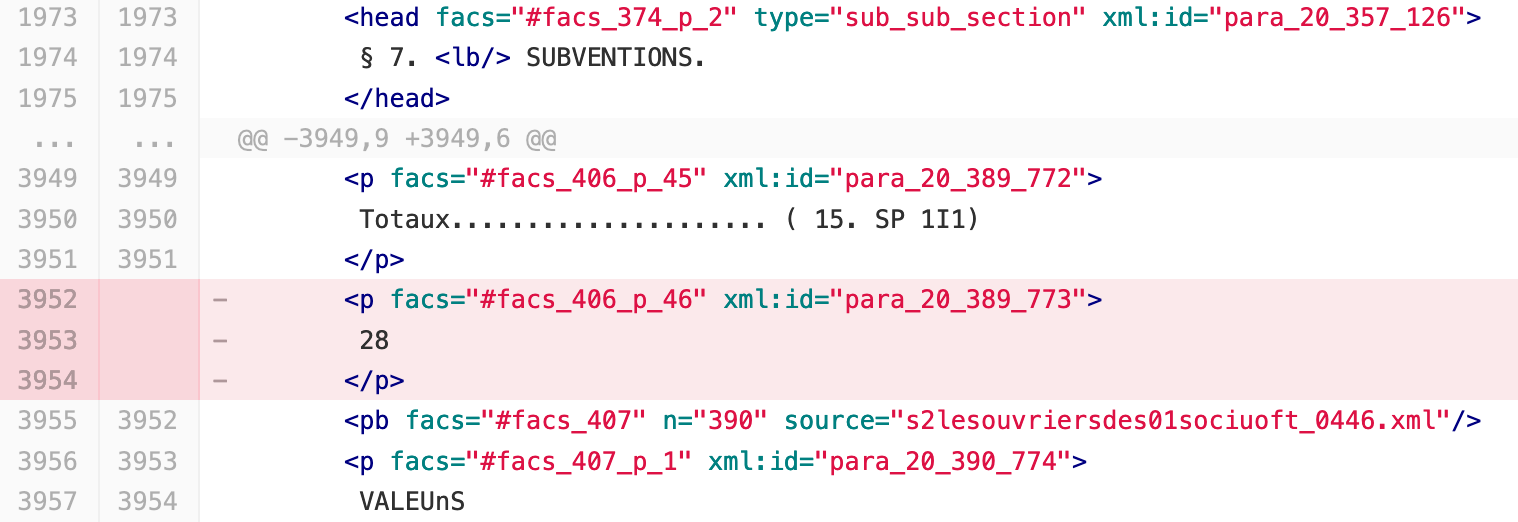
\includegraphics[width=15cm]{img/suppr_num_page.png}
    \caption[Suppression d'un numéro de page]{Suppression du numéro de page 28 dans le fichier  \texttt{s2t1\_chapt\_20.xml} (image du \commit{} sur \gitlab{} --- monographie \no{}53).}
    \label{fig:supprnumpage}
\end{figure}

\begin{figure}
    \centering
    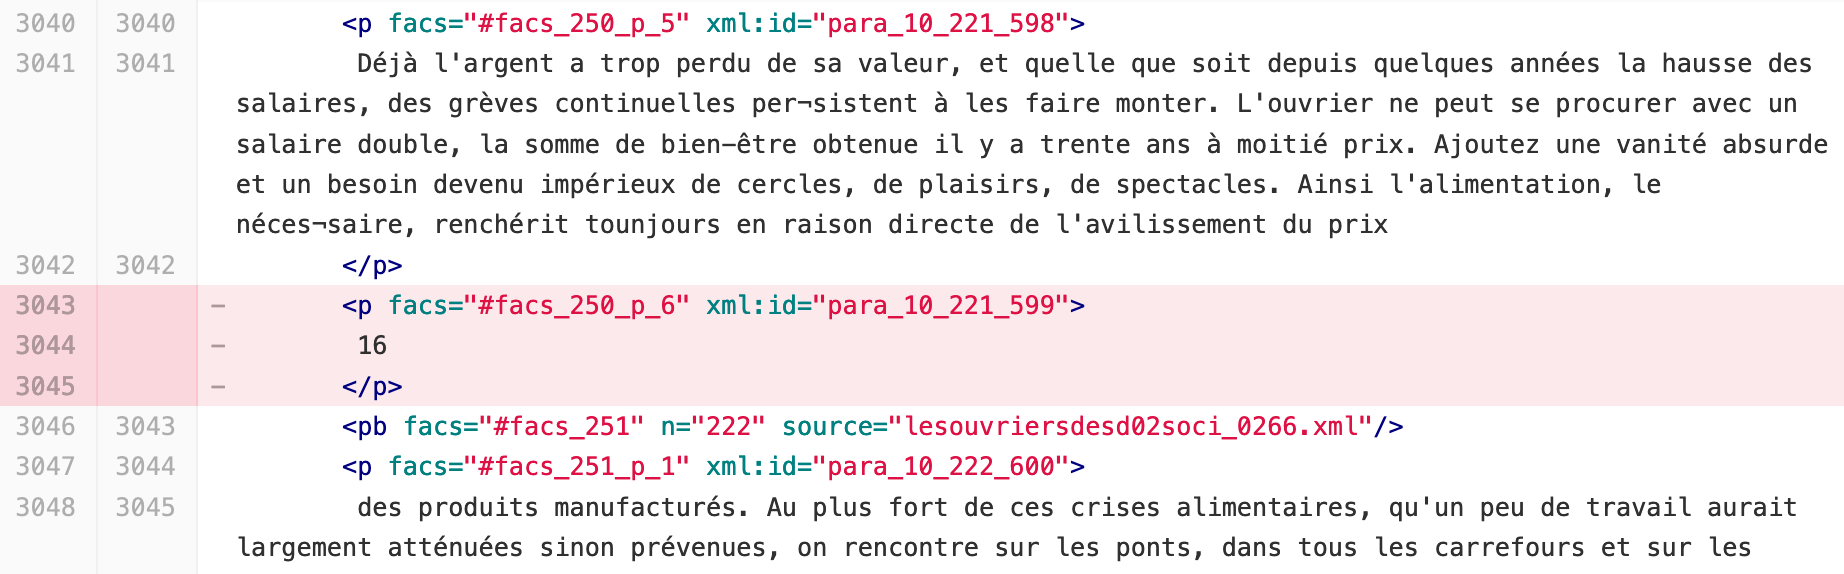
\includegraphics[width=16cm]{img/suppr_num _cahier.png}
    \caption[Suppression d'un numéro de cahier (1)]{Suppression du numéro de cahier 16 dans le fichier  \texttt{s2t2\_chapt\_10.xml} (image du \commit{} sur \gitlab{} --- monographie \no{}59, page 221).}
    \label{fig:suppnumcahier}
\end{figure}

\begin{figure}
    \centering
    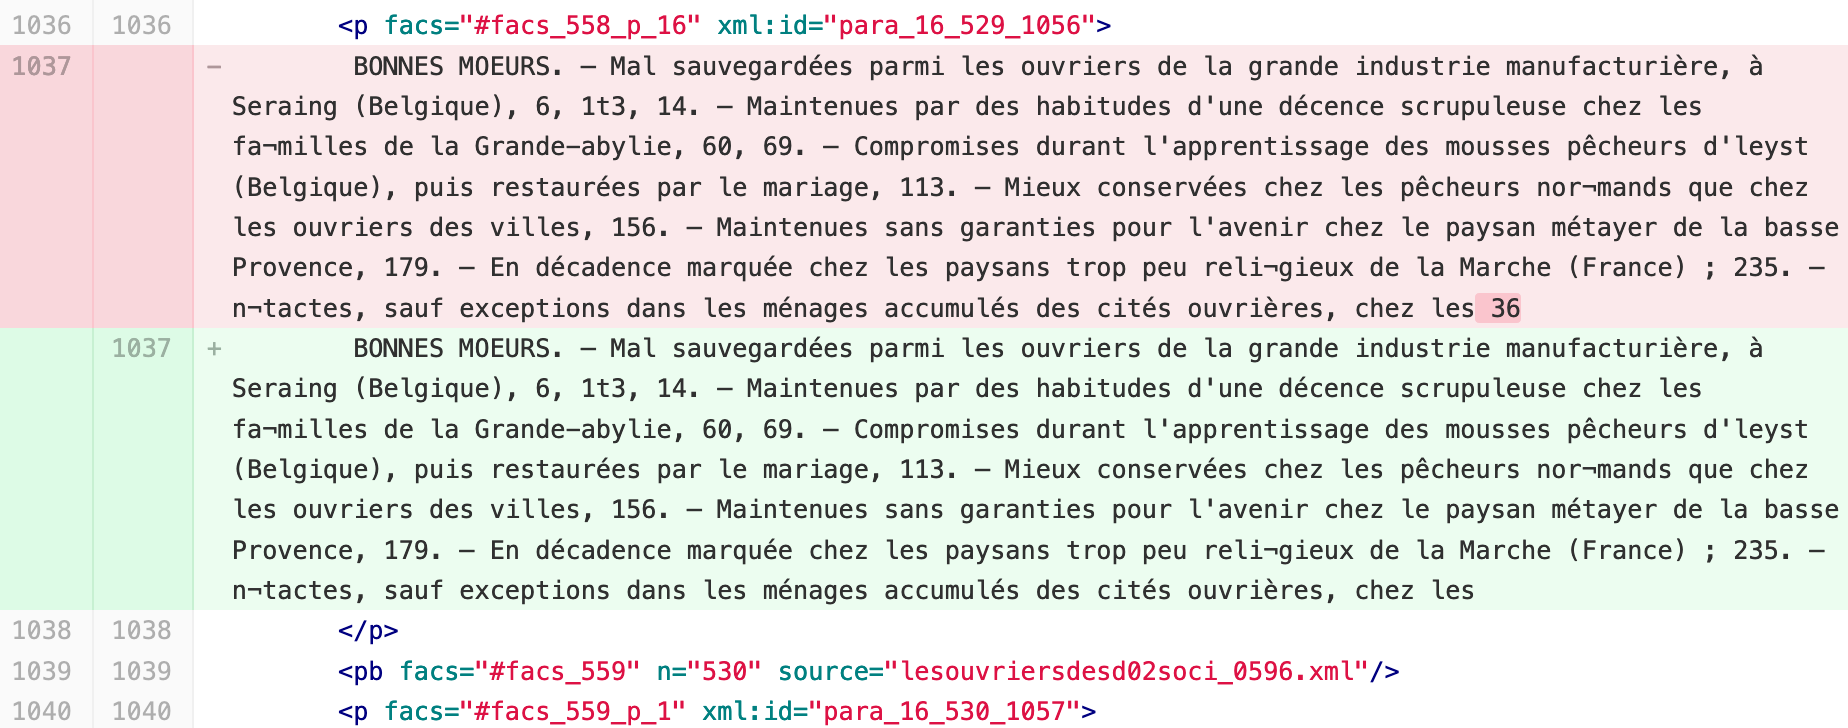
\includegraphics[width=16cm]{img/suppr_num _cahier_visuel.png}
    \caption[Suppression d'un numéro de cahier (2)]{Suppression du numéro de cahier 36 dans le fichier  \texttt{s2t2\_chapt\_10.xml} après un contrôle visuel (image du \commit{} sur \gitlab{} --- table alphabétique et analytique du deuxième volume de la deuxième série, page 529).}
    \label{fig:suppnumcahiervisu}
\end{figure}


\section{Validation du schéma XML-TEI}

Les erreurs de structuration et de transcription traitées dans les quatre premiers niveaux d'encodage, nous pouvions envisager de formaliser le schéma des fichiers. Il s'agit d'établir un document définissant quelles balises peuvent être utilisées dans les fichiers, réglant l'ordre de leur imbrication et arrêtant le nombre et la nature des attributs qui peuvent leur être attachés.

Nous avons choisi d'établir un fichier ODD, entièrement écrit dans une syntaxe XML, qui permet d'établir très précisément les éléments, les séquences d'éléments (nombre et ordre) et leurs attributs. \oxygen{} est capable d'en générer un après avoir analysé un ensemble de fichiers TEI, puis de le transformer en un schéma relaxNG. Ce document relaxNG contient le schéma servant à la validation du fichier TEI, l'ODD étant un fichier XML de documentation et de description de ce schéma. Le document relaxNG est finalement associé au document TEI (\fig{} \ref{fig:tei-odd-rng}), une des fonctionnalités d'\oxygen{} permettant de contrôler à tout moment la validité du code par rapport au schéma.

\begin{figure}[ht]
    \centering
    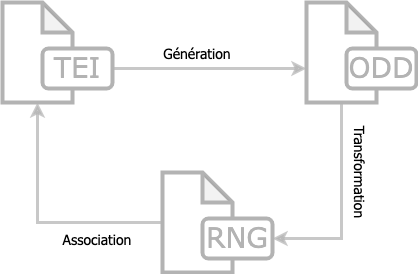
\includegraphics[width=9cm]{img/tei-odd-rng.png}
    \caption{Schématisation du processus de validation à l'aide d'une ODD.}
    \label{fig:tei-odd-rng}
\end{figure}

Le document ODD est généré automatiquement par \oxygen{} grâce au scénario de transformation du Consortium TEI intitulé \textit{oddbyexample}. Il s'agit d'une feuille de style XSL qui, appliquée à un document TEI, analyse l'ensemble des balises et leurs attributs pour les comparer aux préconisations de la TEI\footnote{\textit{The XSLT stylesheet which traverses a nominated directory tree looking for *.xml files which have <TEI> or <teiCorpus> root elements. It analyzes the collection of elements and attributes in the resulting corpus, and compares that to the whole of TEI P5} : \textit{oddbyexample} sur le \textit{TEI Wiki} (\url{https://wiki.tei-c.org/index.php/Oddbyexample}, consulté le \today).}. Puis il génère une ODD où les modules TEI sont chargés, les balises et les attributs non-utilisés étant supprimés d'office et les valeurs des attributs collectées et inscrites dans des listes.

\begin{figure}[ht]
    \centering
    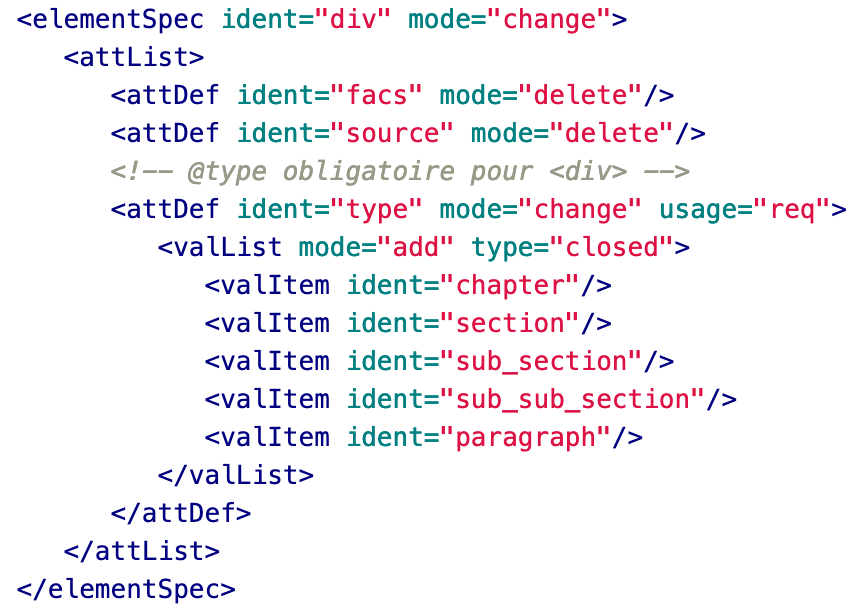
\includegraphics[width=9cm]{img/odd.png}
    \caption[Extrait de l'ODD concernant la balise \texttt{<div>}]{Extrait de l'ODD des \odm{} concernant la balise \texttt{<div>}. Les attributs \texttt{@facs} et \texttt{@source} sont supprimés (\texttt{mode="delete"}), \texttt{@type} est requis (\texttt{usage="req"}) et sa liste de valeurs est close (\texttt{type="closed"}).}
    \label{fig:tei-odd-rng-ex}
\end{figure}

L'utilisateur peut modifier le document obtenu en imposant des règles plus restrictives ou au contraire en en relâchant certaines ; il peut également ajouter des valeurs d'attribut, rendre des attributs obligatoires ou contraindre l'enchaînement de certaines balises. Par exemple, nous avons rendu l'attribut \texttt{@type} obligatoire pour les balises \texttt{<head>} et \texttt{<div>}, et clos la liste de ses valeurs possibles (\fig{} \ref{fig:tei-odd-rng-ex}).

Une ODD peut également être documentée, \cad{} que son rédacteur peut justifier ses choix d'encodage. Disposer d'un schéma et de sa documentation est un élément extrêmement important pour un projet en humanités numériques : c'est en effet une assurance pour la pérennité des données qu'il a rassemblées et structurées. Celles-ci ne sont plus dépendantes des ingénieur(e)s ou des structures institutionnelles et peuvent être réutilisées par d'autres projets\footcite[p. 61]{jolivet}.

Il existe plusieurs possibilités pour permettre la vérification du document TEI. La première et la plus courante est la spécification d'une instruction de traitement au début du document sous la forme suivante : \texttt{<?xml-model href="\#" type="application/xml" schematypens="http://relaxng.org/ns/structure/1.0"?>}, l'attribut \texttt{@href} devant être complété par l'adresse du schéma. Cela suppose bien évidemment que ce schéma soit hébergé, par exemple sur \gitlab. La ligne peut ensuite être ajoutée automatiquement à l'ensemble des fichiers du corpus grâce à la fonction de recherche et de remplacement.

Une autre possibilité est une validation externe, \cad{} qu'un logiciel ou un script vérifie la compatibilité des fichiers par rapport à un schéma qui lui est fourni par l'utilisateur à l'instant \texttt{t} de la validation. C'est une des fonctionnalités du mode \og projet \fg{} d'\oxygen. \timeus{} a cependant souhaité se détacher de tout logiciel, et \textit{a fortiori} d'un logiciel propriétaire, afin de se réserver la possibilité de contrôler la validité de ses fichiers à tout moment.

Le module \texttt{etree} de la librairie Python \texttt{lxml}, qui permet d'analyser un arbre XML, possède un outil répondant parfaitement à ce besoin. En effet, un schéma RNG peut être chargé avec la méthode \texttt{.RelaxNG()}, \texttt{validate()} contrôlant ensuite la validité de tout fichier lui étant donné comme argument par rapport à ce schéma.

La spécificité de ce script est qu'il s'applique à un corpus entier, ce qui avait pour effet d'allonger démesurément son exécution sur notre ordinateur (environ une demi-heure pour traiter une vingtaine de fichiers). Nous avons donc chargé l'ensemble des fichiers, le schéma et le script sur le \textit{cluster} \rioc{} d'Inria, ce qui a considérablement rétréci le temps d'exécution (vingt-quatre minutes au total).

\clearpage

\vspace*{\stretch{0.3}}

La structuration automatique des fichiers des \odm{} par le script \lse{} a donc été contrôlée selon différents niveaux d'encodage.

Sur le plan méthodologique, ce contrôle s'est traduit par plus d'interventions automatiques que manuelles, illustrant le gain de temps que la technologie peut apporter dans la production d'un corpus numérique. Sur le plan scientifique, ces problèmes montrent l'importance de la modélisation d'un corpus physique avant toute entreprise de rédaction d'un script de traitement. Nombre d'erreurs ont en effet été causées par une souplesse très faible d'\lse{} face aux cas particuliers du corpus. Cet effort de modélisation ne peut être mené que si un temps lui est alloué dans le projet.

La modélisation permet également de s'assurer de la pérennité des données. En effet, les fichiers des \odm{} n'existent pas dans le seul objectif de produire une édition numérique, \cad{} d'être mis en scène à travers une interface de consultation. Le processus de valorisation des données de la recherche peut emprunter deux voies différentes. L'une consiste à inscrire ces données dans le temps long et à favoriser leur ré-utilisation grâce à une structuration standardisée et documentée. L'autre entraîne leur publication dans un cadre institutionnel et budgétaire conjoncturel qui, s'il peut produire des résultats visibles rapidement, n'est pas assuré d'être reconduit et pérennisé.

Les fichiers des \odm{} se trouvent face à cette injonction qui, sans être réellement paradoxale, conjugue une obligation --- publier avant la fin du programme ANR \timeus{} --- et une ambition --- assurer la pérennité d'un corpus numérique.

Plusieurs voies sont envisagées pour répondre à ces nécessités. Aucune n'a pu être mise en place au cours de notre stage, mais nous avons mené plusieurs réflexions et quelques actions en leur sens. Nous allons d'abord présenter celles qui concernent les objets graphiques, puis nous intéresser à l'état des transcriptions, avant de conclure sur les différents types d'édition possibles et ce qu'ils impliquent pour les données issues du traitement automatique des fichiers des \odm.

\vspace*{\stretch{1.7}}

\newpage
\thispagestyle{empty}
\mbox{}
\newpage